\documentclass[a4paper]{article}
\usepackage[warn]{mathtext}
\usepackage{graphicx}
\usepackage{wrapfig}
\usepackage{enumitem}
\usepackage[center]{caption}
\usepackage[english, russian]{babel}
\usepackage{amsmath}
\usepackage{amssymb}
\usepackage{geometry}
\usepackage{longtable}
\usepackage{booktabs}
\setcounter{totalnumber}{5}

\geometry{verbose, a4paper, tmargin=2cm, bmargin=2cm, lmargin=2.0cm, rmargin=2.0cm}

\begin{document}
	
	\begin{titlepage}
		\centering
		{\scshape\Large МОСКОВСКИЙ ФИЗИКО-ТЕХНИЧЕСКИЙ ИНСТИТУТ \\
			(НАЦИОНАЛЬНЫЙ ИССЛЕДОВАТЕЛЬСКИЙ УНИВЕРСИТЕТ)\\
			Физтех-школа аэрокосмических технологий}
		
		\vspace{4cm}
		{\LARGE Отчет о выполнении лабораторной работы 3.5.1}
		\vspace{1cm}
		
		{\huge\bf Изучение плазмы газового разряда в неоне}
		
		\vspace{1cm}
		\vfill
		
		\begin{flushright}
			{\LARGE Губарев Никита, Б03-502}
		\end{flushright}
		\vfill 
		\today
	\end{titlepage}
	
	\tableofcontents
	
	\section{Аннотация}
	
	\textbf{Цель работы:} изучение вольт-амперной характеристики тлеющего разряда и зондовых характеристик плазмы; определение концентрации и температуры электронов, плазменной частоты, поляризационной длины, дебаевского радиуса экранирования и степени ионизации плазмы.
	
	\textbf{В работе используются:} стеклянная газоразрядная трубка с неоном $^{22}$Ne при давлении $P \approx 2$ мм рт.~ст.; высоковольтный источник питания ВИП ($0$--$5$ кВ); источник постоянного тока GPS ($0$--$30$ В); делитель напряжения $(R_1+R_2)/R_2 = 10$; балластный резистор $R_б \approx 450$ кОм; потенциометр $R$; мультиметры GDM; двойной зонд (молибден, $d = (0{,}2 \pm 0{,}1)$ мм, $l = (5{,}2 \pm 0{,}1)$ мм); переключатели $\Pi_1$, $\Pi_2$.
	
	\section{Теоретические сведения}
	
	\subsection{Основные параметры плазмы}
	
	\textbf{Плазма} — ионизованный газ, размеры которого существенно превосходят дебаевский радиус экранирования $r_D$. Основные характеристики:
	
	\subsubsection{Плазменная (ленгмюровская) частота}
	\begin{equation}
		\omega_p = \sqrt{\frac{4\pi n_e e^2}{m_e}} = 5{,}6\cdot 10^4 \sqrt{n_e} \ \text{рад/с} \quad (\text{СГС}, \ n_e \ \text{в см}^{-3}).
		\label{eq:omega_p}
	\end{equation}
	
	\subsubsection{Дебаевские длины}
	Электронная поляризационная длина:
	\begin{equation}
		r_{De} = \sqrt{\frac{k_B T_e}{4\pi n_e e^2}}.
		\label{eq:rDe}
	\end{equation}
	Радиус экранирования (при $T_e \gg T_i$):
	\begin{equation}
		r_D \approx r_{Di} = \sqrt{\frac{k_B T_i}{4\pi n_i e^2}}.
		\label{eq:rD}
	\end{equation}
	
	\subsubsection{Число частиц в дебаевской сфере}
	\begin{equation}
		N_D = \frac{4}{3}\pi r_D^3 n_i, \quad N_D \gg 1 \text{ — идеальная плазма}.
		\label{eq:ND}
	\end{equation}
	
	\subsubsection{Степень ионизации}
	\begin{equation}
		\alpha = n_i / n, \qquad n = P/(k_B T_i).
	\end{equation}
	
	\subsection{Метод двойного зонда}
	
	Двойной зонд — две одинаковые проволочки, между которыми создаётся разность потенциалов $U$. Ток в цепи:
	\begin{equation}
		I = I_{in} \tanh\!\left(\frac{eU}{2k_BT_e}\right),
		\label{eq:double_probe}
	\end{equation}
	где $I_{in}$ — ионный ток насыщения. При $U \to 0$:
	\[
	\left.\frac{dI}{dU}\right|_{U=0} = \frac{e I_{in}}{2k_BT_e}
	\quad\Rightarrow\quad
	k_BT_e = \frac{1}{2}\frac{I_{in}}{(dI/dU)|_{U=0}}.
	\]
	
	Формула Бома:
	\begin{equation}
		I_{in} = 0{,}4\, n_e e S \sqrt{\frac{2k_BT_e}{m_i}},
		\label{eq:bohm}
	\end{equation}
	где $S = \pi d l$ — площадь поверхности зонда.
	
	\section{Экспериментальная установка}
	
	Схема установки приведена на рис.~\ref{fig:setup}. Стеклянная газоразрядная трубка наполнена $^{22}$Ne при $P \approx 2$ мм рт.~ст., имеет полый холодный катод, три анода и геттерный узел. Катод и один из анодов (I или II) через $\Pi_1$ подключаются к ВИП ($0$--$5$ кВ) через балластный резистор $R_б \approx 450$ кОм. Ток разряда — амперметр $A_1$; напряжение — вольтметр $V_1$ через делитель 1:10.
	
	Двойной зонд (Mo, $d = 0{,}2$ мм, $l = 5{,}2$ мм) подключён к источнику GPS ($0$--$30$ В) через потенциометр $R$. Напряжение на зонде — вольтметр $V_2$, ток — мультиметр $A_2$. Переключатель $\Pi_2$ меняет полярность.
	
	\begin{figure}[h]
		\centering
		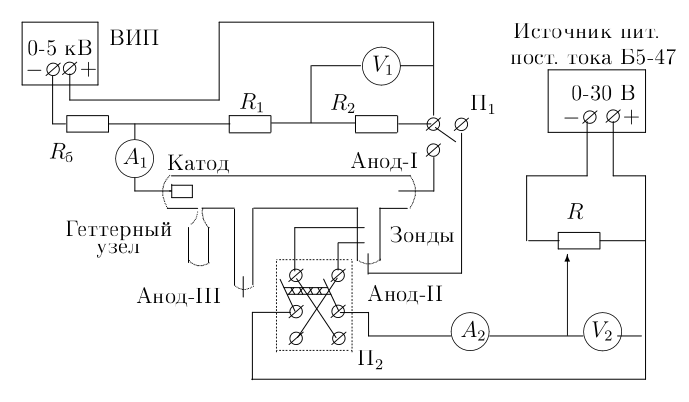
\includegraphics[width=0.95\textwidth]{setup.png}
		\caption{Схема установки}
		\label{fig:setup}
	\end{figure}
	
	\section{Методика измерений}
	
	\subsection{ВАХ разряда}
	\begin{enumerate}
		\item $\Pi_1$ — <<Анод-I>>; ручка ВИП на минимум.
		\item Плавно увеличивая напряжение, определить $U_{\text{заж}}$.
		\item Снять ВАХ $I_p(U_p)$ при $I_p$ от $0{,}5$ до $5$ мА при нарастании и убывании тока.
	\end{enumerate}
	
	\subsection{Зондовые характеристики}
	\begin{enumerate}
		\item ВИП → 0; $\Pi_1$ → <<Анод-II>>; $\Pi_2$ → <<+>>.
		\item Установить $I_p \approx 5$ мА, $U_{\text{GPS}} \approx 25$ В.
		\item Снять $I_3(U_3)$ от $+25$ до $-25$ В. Шаг 3 В при $|U|>10$ В, 2 В при $|U|<10$ В.
		\item Меняя полярность $\Pi_2$, снять ветвь при $U < 0$.
		\item Повторить при $I_p = 3{,}0$ и $1{,}5$ мА.
	\end{enumerate}
	
	\section{Результаты измерений}
	
	\subsection{Параметры}
	
	\begin{table}[h]
		\centering
		\caption{Параметры установки (погрешности — по последнему значащему знаку)}
		\label{tab:params}
		\begin{tabular}{|l|c|c|}
			\hline
			Параметр & Обозначение & Значение \\
			\hline
			Диаметр зонда & $d$ & $(0{,}2 \pm 0{,}1)$ мм \\
			\hline
			Длина зонда & $l$ & $(5{,}2 \pm 0{,}1)$ мм \\
			\hline
			Площадь зонда & $S = \pi d l$ & $(3{,}27 \pm 1{,}7)\cdot 10^{-6}$ м² \\
			\hline
			Давление неона & $P$ & 2 мм рт.~ст. \\
			\hline
			Масса иона неона & $m_i$ & $3{,}65\cdot 10^{-26}$ кг \\
			\hline
		\end{tabular}
	\end{table}
	
	\subsection{ВАХ разряда}
	
	Напряжение зажигания: $U_{\text{заж}} = (2140{,}000 \pm 0{,}001)$ В. После зажигания напряжение разряда резко падает и далее лежит в диапазоне 185--350 В.
	
	\begin{table}[h]
		\centering
		\caption{ВАХ разряда. Значения $U_p$ — показания мультиметра, умноженные на 10. Погрешности: $\delta U_p = 0{,}1$ В, $\delta I_p = 0{,}0001$ мА.}
		\label{tab:VAC}
		\begin{tabular}{|c|c||c|c|}
			\hline
			\multicolumn{2}{|c||}{Нарастание} & \multicolumn{2}{c|}{Убывание} \\
			\hline
			$U_p$, В & $I_p$, мА & $U_p$, В & $I_p$, мА \\
			\hline
			$349{,}92 \pm 0{,}10$ & $0{,}5409$ & $186{,}00 \pm 0{,}10$ & $4{,}8384$ \\
			$341{,}18 \pm 0{,}10$ & $0{,}8118$ & $189{,}75 \pm 0{,}10$ & $4{,}4253$ \\
			$328{,}53 \pm 0{,}10$ & $1{,}0885$ & $195{,}76 \pm 0{,}10$ & $4{,}0370$ \\
			$301{,}60 \pm 0{,}10$ & $1{,}2976$ & $197{,}71 \pm 0{,}10$ & $3{,}7497$ \\
			$268{,}63 \pm 0{,}10$ & $1{,}6015$ & $200{,}56 \pm 0{,}10$ & $3{,}4466$ \\
			$254{,}28 \pm 0{,}10$ & $1{,}8553$ & $211{,}28 \pm 0{,}10$ & $3{,}0404$ \\
			$240{,}83 \pm 0{,}10$ & $2{,}1580$ & $224{,}86 \pm 0{,}10$ & $2{,}6517$ \\
			$229{,}50 \pm 0{,}10$ & $2{,}5116$ & $245{,}64 \pm 0{,}10$ & $2{,}0325$ \\
			$221{,}92 \pm 0{,}10$ & $2{,}7408$ & $264{,}25 \pm 0{,}10$ & $1{,}6676$ \\
			$211{,}06 \pm 0{,}10$ & $3{,}0531$ & $331{,}59 \pm 0{,}10$ & $1{,}0515$ \\
			$200{,}71 \pm 0{,}10$ & $3{,}4761$ & $339{,}11 \pm 0{,}10$ & $0{,}8764$ \\
			$197{,}38 \pm 0{,}10$ & $3{,}9168$ & $345{,}60 \pm 0{,}10$ & $0{,}6741$ \\
			$191{,}35 \pm 0{,}10$ & $4{,}3513$ & $350{,}70 \pm 0{,}10$ & $0{,}5193$ \\
			$186{,}60 \pm 0{,}10$ & $4{,}7599$ & & \\
			$184{,}92 \pm 0{,}10$ & $4{,}9737$ & & \\
			\hline
		\end{tabular}
	\end{table}
	
	\subsection{Зондовые характеристики}
	
	Погрешности прямых измерений: $\delta U_3 = 0{,}001$ В, $\delta I_3 = 0{,}01$ мкА.
	
	\begin{longtable}{|c|c||c|c||c|c|}
		\caption{Зондовые характеристики при трёх токах разряда}
		\label{tab:probes} \\
		\hline
		\multicolumn{2}{|c||}{$I_p = 4{,}9877$ мА} & \multicolumn{2}{c||}{$I_p = 3{,}0041$ мА} & \multicolumn{2}{c|}{$I_p = 1{,}5041$ мА} \\
		\hline
		$U_3$, В & $I_3$, мкА & $U_3$, В & $I_3$, мкА & $U_3$, В & $I_3$, мкА \\
		\hline
		\endfirsthead
		\hline
		$U_3$, В & $I_3$, мкА & $U_3$, В & $I_3$, мкА & $U_3$, В & $I_3$, мкА \\
		\hline
		\endhead
		25{,}013 & 109{,}04 & 25{,}022 & 63{,}77 & 25{,}024 & 31{,}99 \\
		22{,}033 & 106{,}55 & 22{,}059 & 61{,}92 & 22{,}023 & 30{,}87 \\
		19{,}076 & 103{,}64 & 19{,}007 & 60{,}04 & 19{,}016 & 29{,}78 \\
		16{,}113 & 99{,}02 & 16{,}048 & 57{,}80 & 16{,}059 & 28{,}64 \\
		13{,}055 & 91{,}52 & 13{,}050 & 54{,}22 & 13{,}006 & 27{,}02 \\
		10{,}020 & 80{,}22 & 10{,}008 & 47{,}85 & 10{,}030 & 24{,}20 \\
		8{,}034 & 70{,}55 & 8{,}011 & 41{,}66 & 8{,}009 & 21{,}27 \\
		6{,}007 & 58{,}98 & 6{,}021 & 33{,}70 & 6{,}047 & 17{,}38 \\
		4{,}0115 & 46{,}38 & 4{,}0427 & 24{,}03 & 4{,}031 & 12{,}16 \\
		2{,}0486 & 32{,}82 & 2{,}0250 & 12{,}68 & 2{,}0011 & 5{,}68 \\
		1{,}0674 & 24{,}80 & 1{,}0000 & 6{,}25 & 1{,}0071 & 2{,}07 \\
		0{,}5316 & 21{,}14 & 0{,}5198 & 3{,}23 & 0{,}5408 & 0{,}37 \\
		$-0{,}4975$ & $-32{,}37$ & $-0{,}5126$ & $-11{,}33$ & $-0{,}4644$ & $-4{,}40$ \\
		$-1{,}0407$ & $-36{,}31$ & $-1{,}030$ & $-14{,}66$ & $-1{,}0500$ & $-6{,}54$ \\
		$-2{,}0612$ & $-44{,}30$ & $-2{,}0178$ & $-20{,}62$ & $-2{,}0763$ & $-10{,}17$ \\
		$-4{,}0126$ & $-57{,}97$ & $-4{,}0178$ & $-31{,}82$ & $-3{,}9505$ & $-16{,}18$ \\
		$-6{,}033$ & $-70{,}69$ & $-5{,}998$ & $-41{,}46$ & $-4{,}0612$ & $-16{,}51$ \\
		$-7{,}994$ & $-81{,}97$ & $-8{,}034$ & $-49{,}52$ & $-6{,}102$ & $-21{,}72$ \\
		$-10{,}048$ & $-92{,}17$ & $-10{,}030$ & $-55{,}70$ & $-8{,}174$ & $-25{,}80$ \\
		$-13{,}085$ & $-104{,}02$ & $-13{,}047$ & $-62{,}04$ & $-10{,}012$ & $-28{,}48$ \\
		$-16{,}206$ & $-112{,}48$ & $-16{,}088$ & $-65{,}84$ & $-13{,}013$ & $-31{,}44$ \\
		$-19{,}178$ & $-117{,}86$ & $-19{,}009$ & $-68{,}19$ & $-16{,}014$ & $-33{,}15$ \\
		$-22{,}047$ & $-121{,}36$ & $-22{,}040$ & $-70{,}23$ & $-19{,}057$ & $-34{,}46$ \\
		$-25{,}023$ & $-124{,}31$ & $-25{,}021$ & $-72{,}19$ & $-22{,}048$ & $-35{,}70$ \\
		& & & & $-25{,}025$ & $-37{,}01$ \\
		\hline
	\end{longtable}
	
	\section{Обработка результатов}
	
	\subsection{ВАХ разряда}
	
	По данным табл.~\ref{tab:VAC} на рис.~\ref{fig:VAC} построена ВАХ. Видны два участка: \textbf{поднормальный (аномальный) тлеющий разряд} ($I_p < 3$ мА, напряжение быстро падает с ростом тока) и \textbf{нормальный тлеющий разряд} ($I_p \approx 3$--$5$ мА, пологий участок).
	
	Максимальное дифференциальное сопротивление:
	\[
	R_{\text{диф}} = -\left.\frac{dU_p}{dI_p}\right|_{\max}
	= \frac{U_{p,3}-U_{p,2}}{I_{p,3}-I_{p,2}}
	= \frac{328{,}53 - 301{,}60}{1{,}0885 - 1{,}2976} \ \frac{\text{В}}{\text{мА}}
	\approx 1{,}29\cdot 10^5 \ \text{Ом}
	\approx 1{,}3\cdot 10^2 \ \text{кОм}.
	\]
	
	Погрешность:
	\[
	\delta R_{\text{диф}} = R_{\text{диф}}\sqrt{\left(\frac{\delta U_p}{\Delta U_p}\right)^2 + \left(\frac{\delta I_p}{\Delta I_p}\right)^2}
	\approx R_{\text{диф}}\sqrt{\left(\frac{0{,}1}{26{,}93}\right)^2 + \left(\frac{0{,}0001}{0{,}2091}\right)^2} \approx 0{,}005 \ R_{\text{диф}}.
	\]
	
	Итог: $R_{\text{диф}} = (1{,}29 \pm 0{,}01)\cdot 10^5$ Ом $\approx 130$ кОм.
	
	Дифференциальное сопротивление на порядок меньше балластного $R_б = 450$ кОм — это нормально для рабочей точки в области поднормального тлеющего разряда.
	
	\begin{figure}[h]
		\centering
		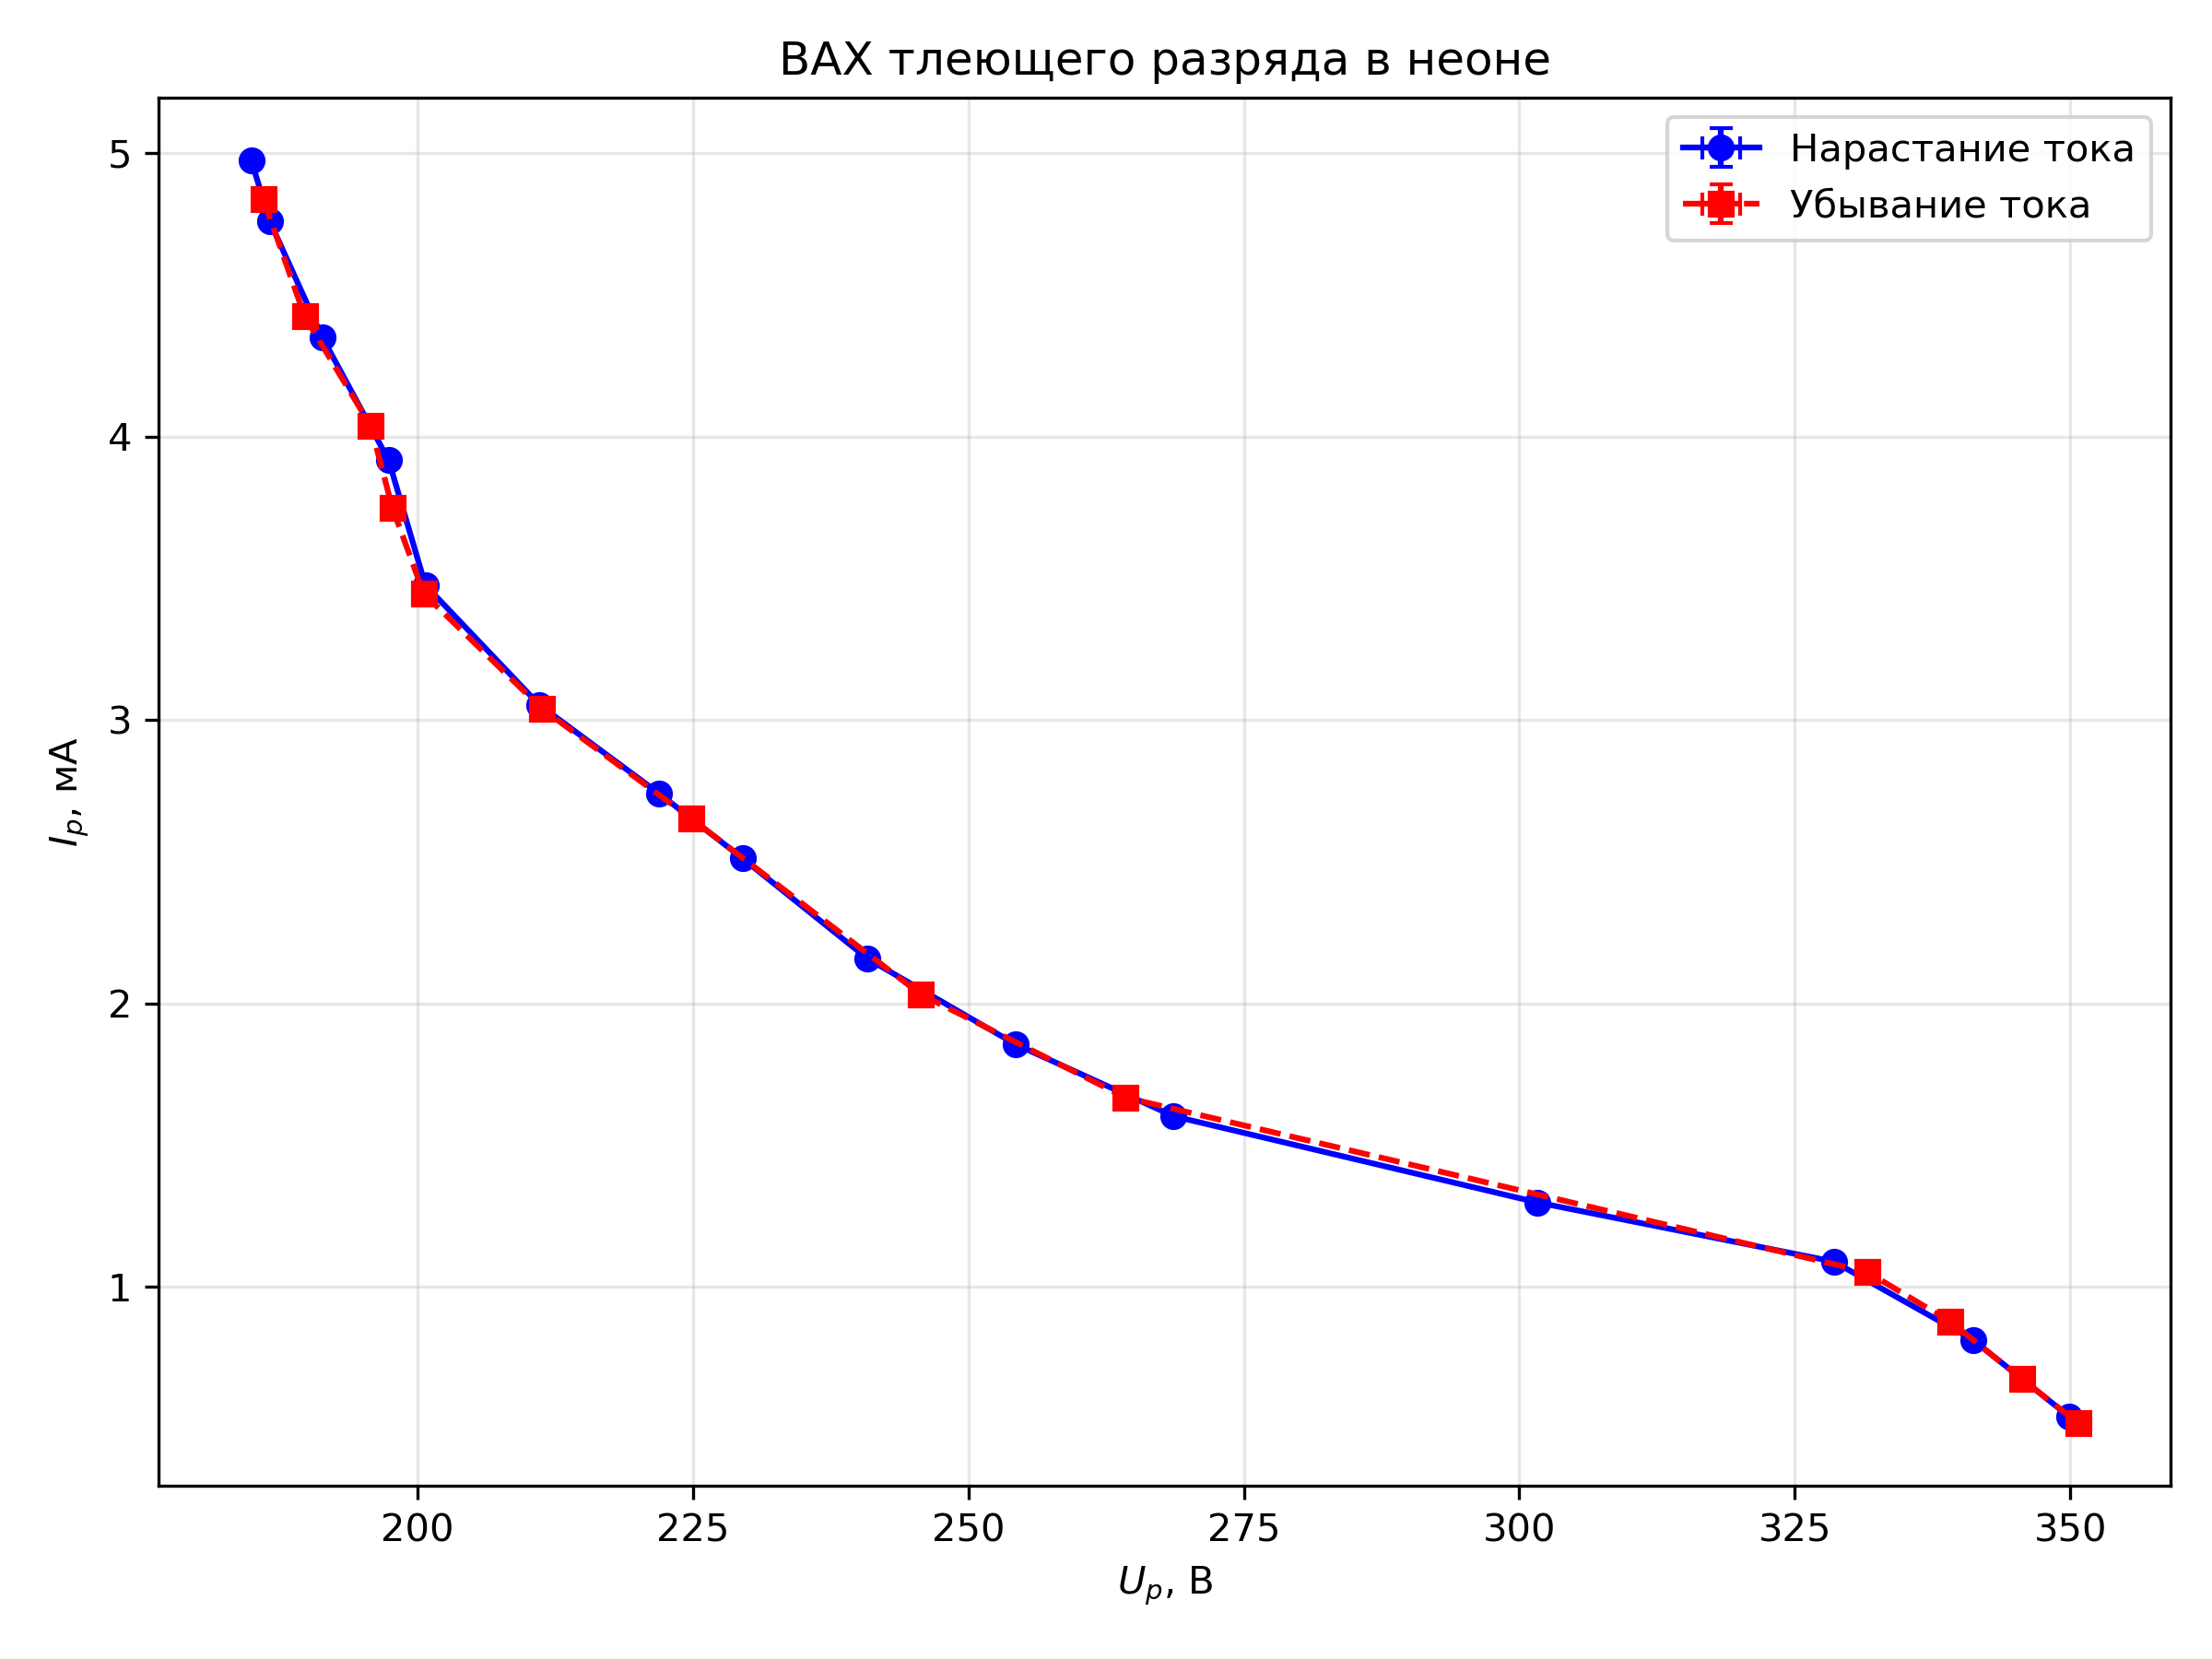
\includegraphics[width=0.85\textwidth]{vac.png}
		\caption{Вольт-амперная характеристика тлеющего разряда в неоне}
		\label{fig:VAC}
	\end{figure}
	
	\subsection{Метод обработки зондовых характеристик}
	
	\textbf{Асимптоты.} Проводятся две прямые: по первым 4 точкам при $U>0$ ($I_+ = k_+ U + b_+$) и по последним 4 точкам при $U<0$ ($I_- = k_- U + b_-$). Пересечения с осью $U=0$ дают $b_+$ и $b_-$, откуда
	\[
	I_{\text{center}} = \frac{b_+ + b_-}{2}, \qquad I_{in} = \frac{b_+ - b_-}{2}.
	\]
	
	\textbf{Наклон в нуле.} После центрирования ($I_c = I - I_{\text{center}}$) наклон определяется линейной регрессией по точкам $|I_c| < I_{in}/2$.
	
	\textbf{Температура электронов.}
	\[
	k_BT_e = \frac{1}{2}\frac{I_{in}}{(dI/dU)|_{U=0}}.
	\]
	
	\begin{figure}[h]
		\centering
		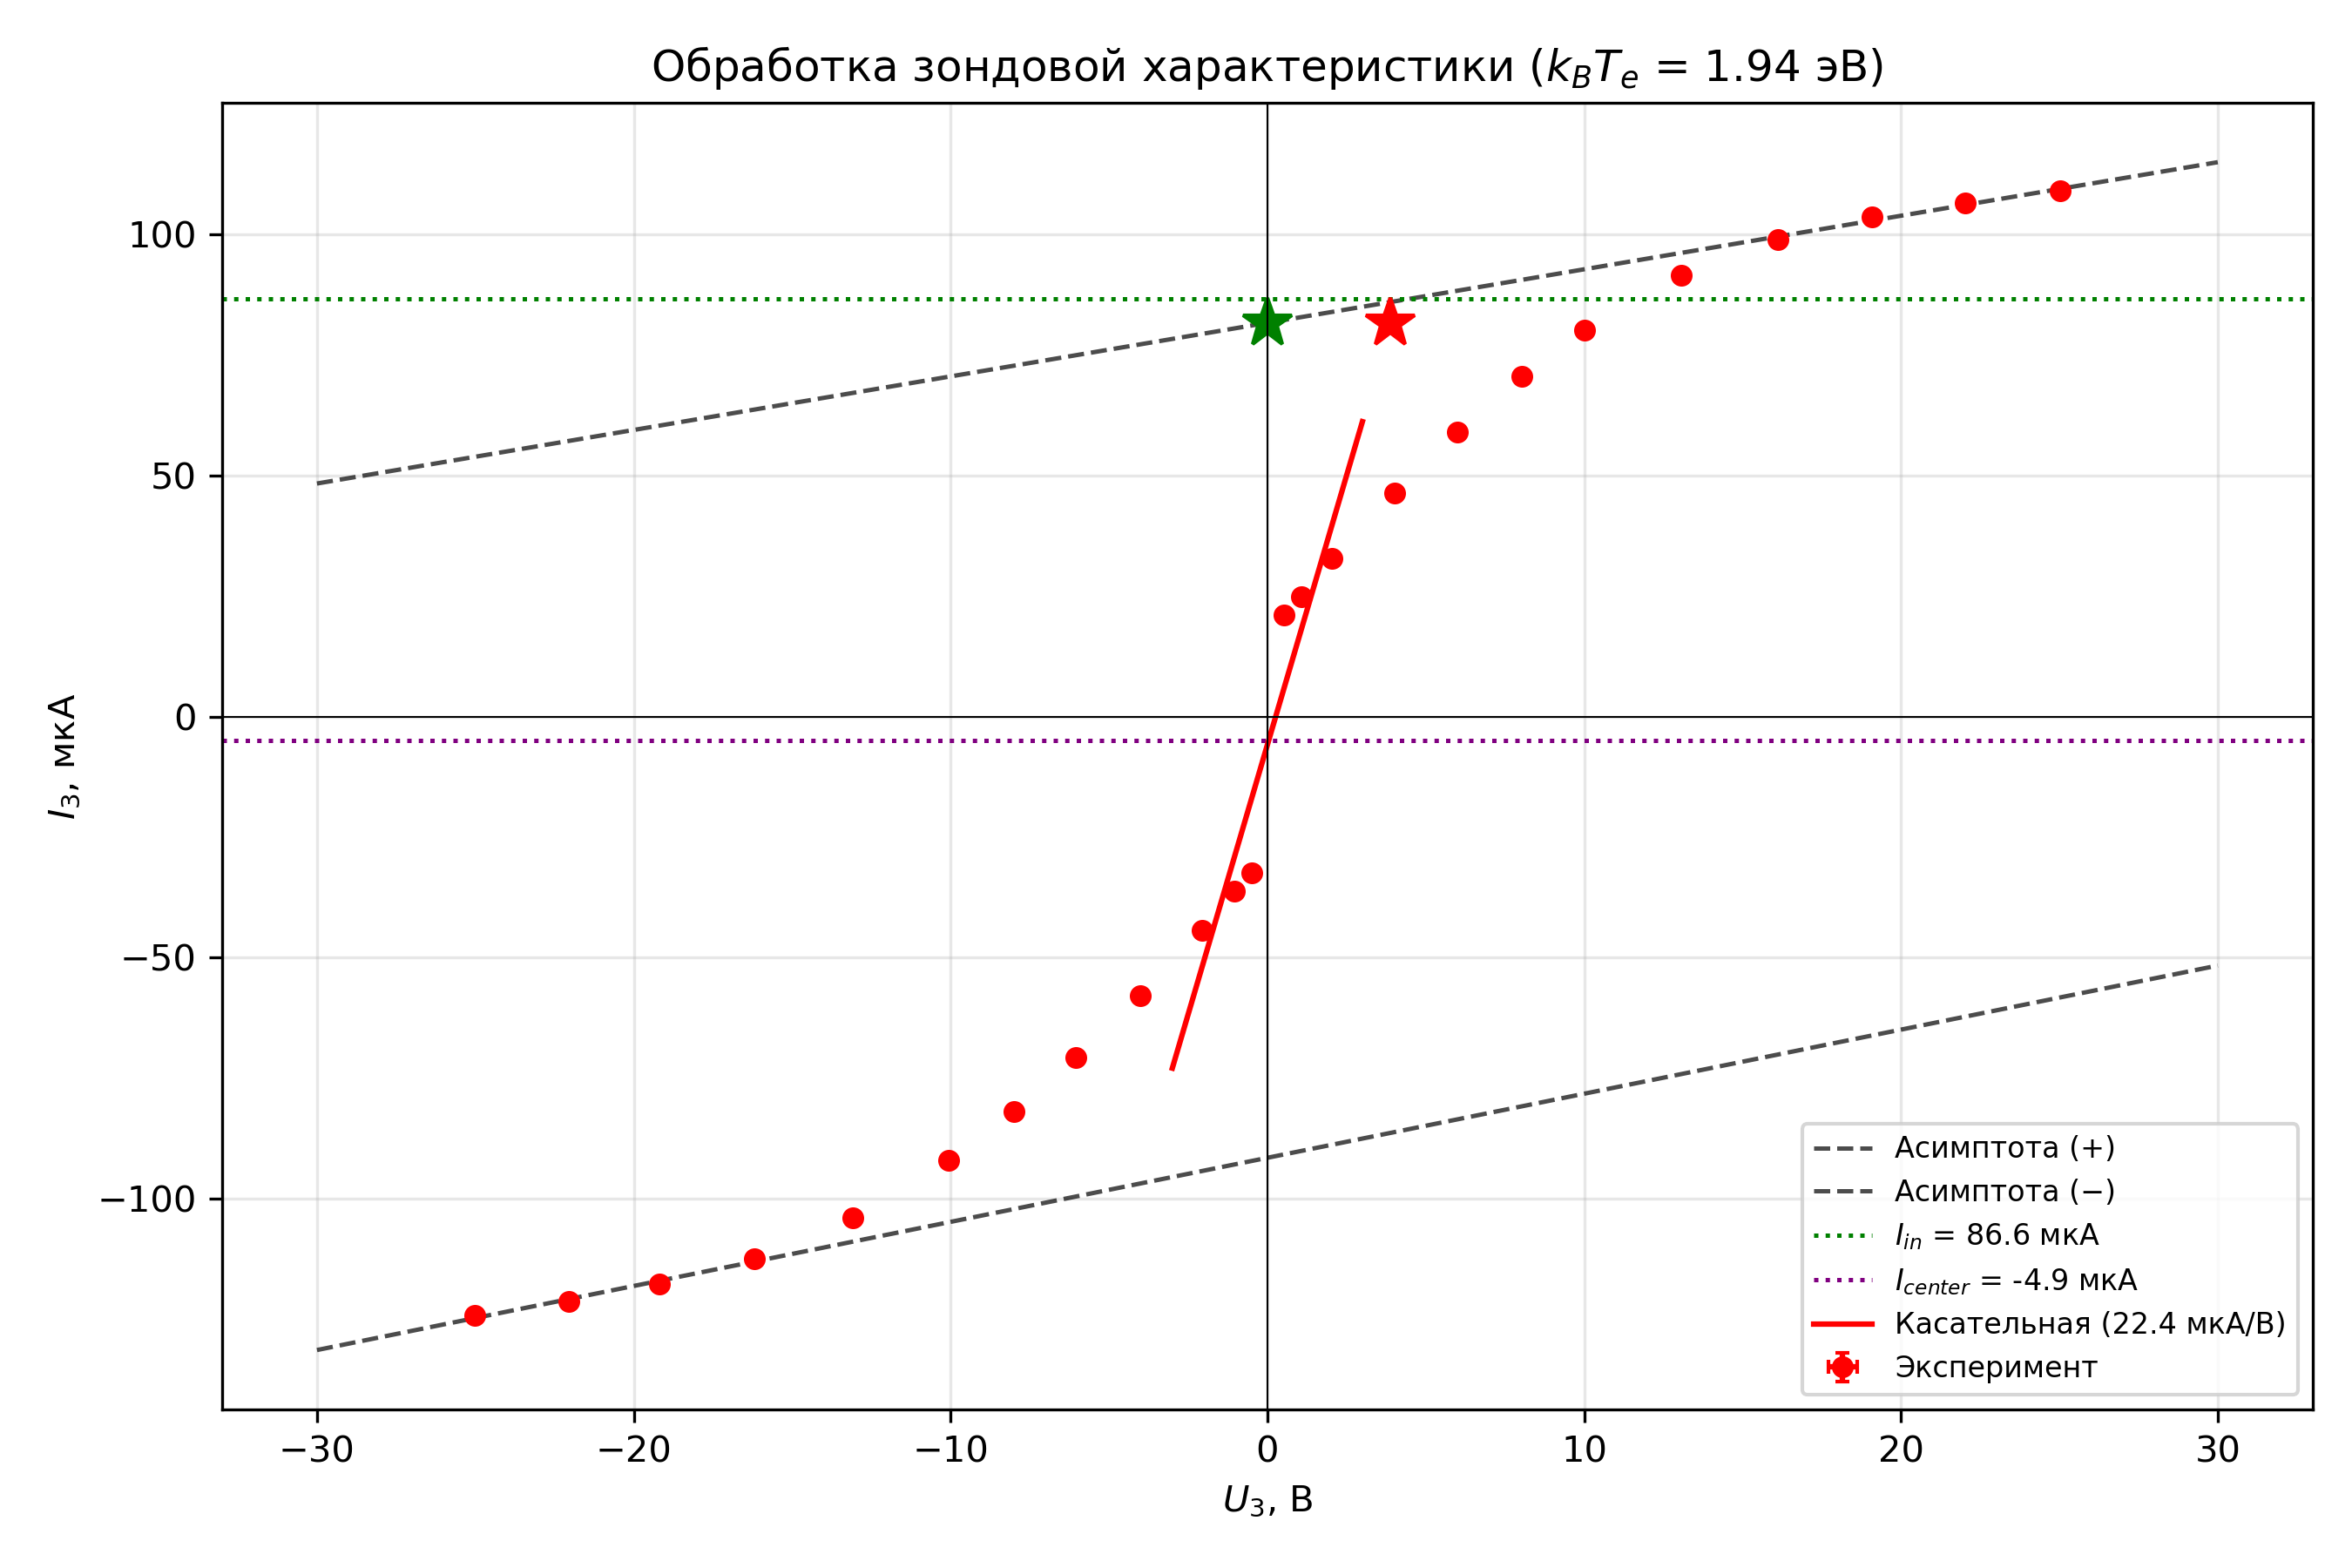
\includegraphics[width=0.9\textwidth]{probe_analysis.png}
		\caption{Обработка зондовой характеристики для $I_p = 4{,}99$ мА: асимптоты, горизонталь $I_{in}$, касательная в нуле, точки 1 и 2}
		\label{fig:probe_analysis}
	\end{figure}
	
	\subsection{Параметры зондовых характеристик}
	
	\begin{table}[h]
		\centering
		\caption{Параметры зондовых характеристик}
		\label{tab:probe_params}
		\begin{tabular}{|c|c|c|c|c|}
			\hline
			$I_p$, мА & $I_{\text{center}}$, мкА & $I_{in}$, мкА & $(dI/dU)|_0$, мкА/В & $k_BT_e$, эВ \\
			\hline
			$4{,}9877$ & $\approx 8 \pm 1$ & $90 \pm 5$ & $50 \pm 5$ & $0{,}9 \pm 0{,}15$ \\
			\hline
			$3{,}0041$ & $\approx -4 \pm 1$ & $53 \pm 3$ & $15 \pm 1{,}5$ & $1{,}8 \pm 0{,}27$ \\
			\hline
			$1{,}5041$ & $\approx -3 \pm 1$ & $26 \pm 2$ & $5 \pm 0{,}5$ & $2{,}6 \pm 0{,}4$ \\
			\hline
		\end{tabular}
	\end{table}
	
	\begin{figure}[h]
		\centering
		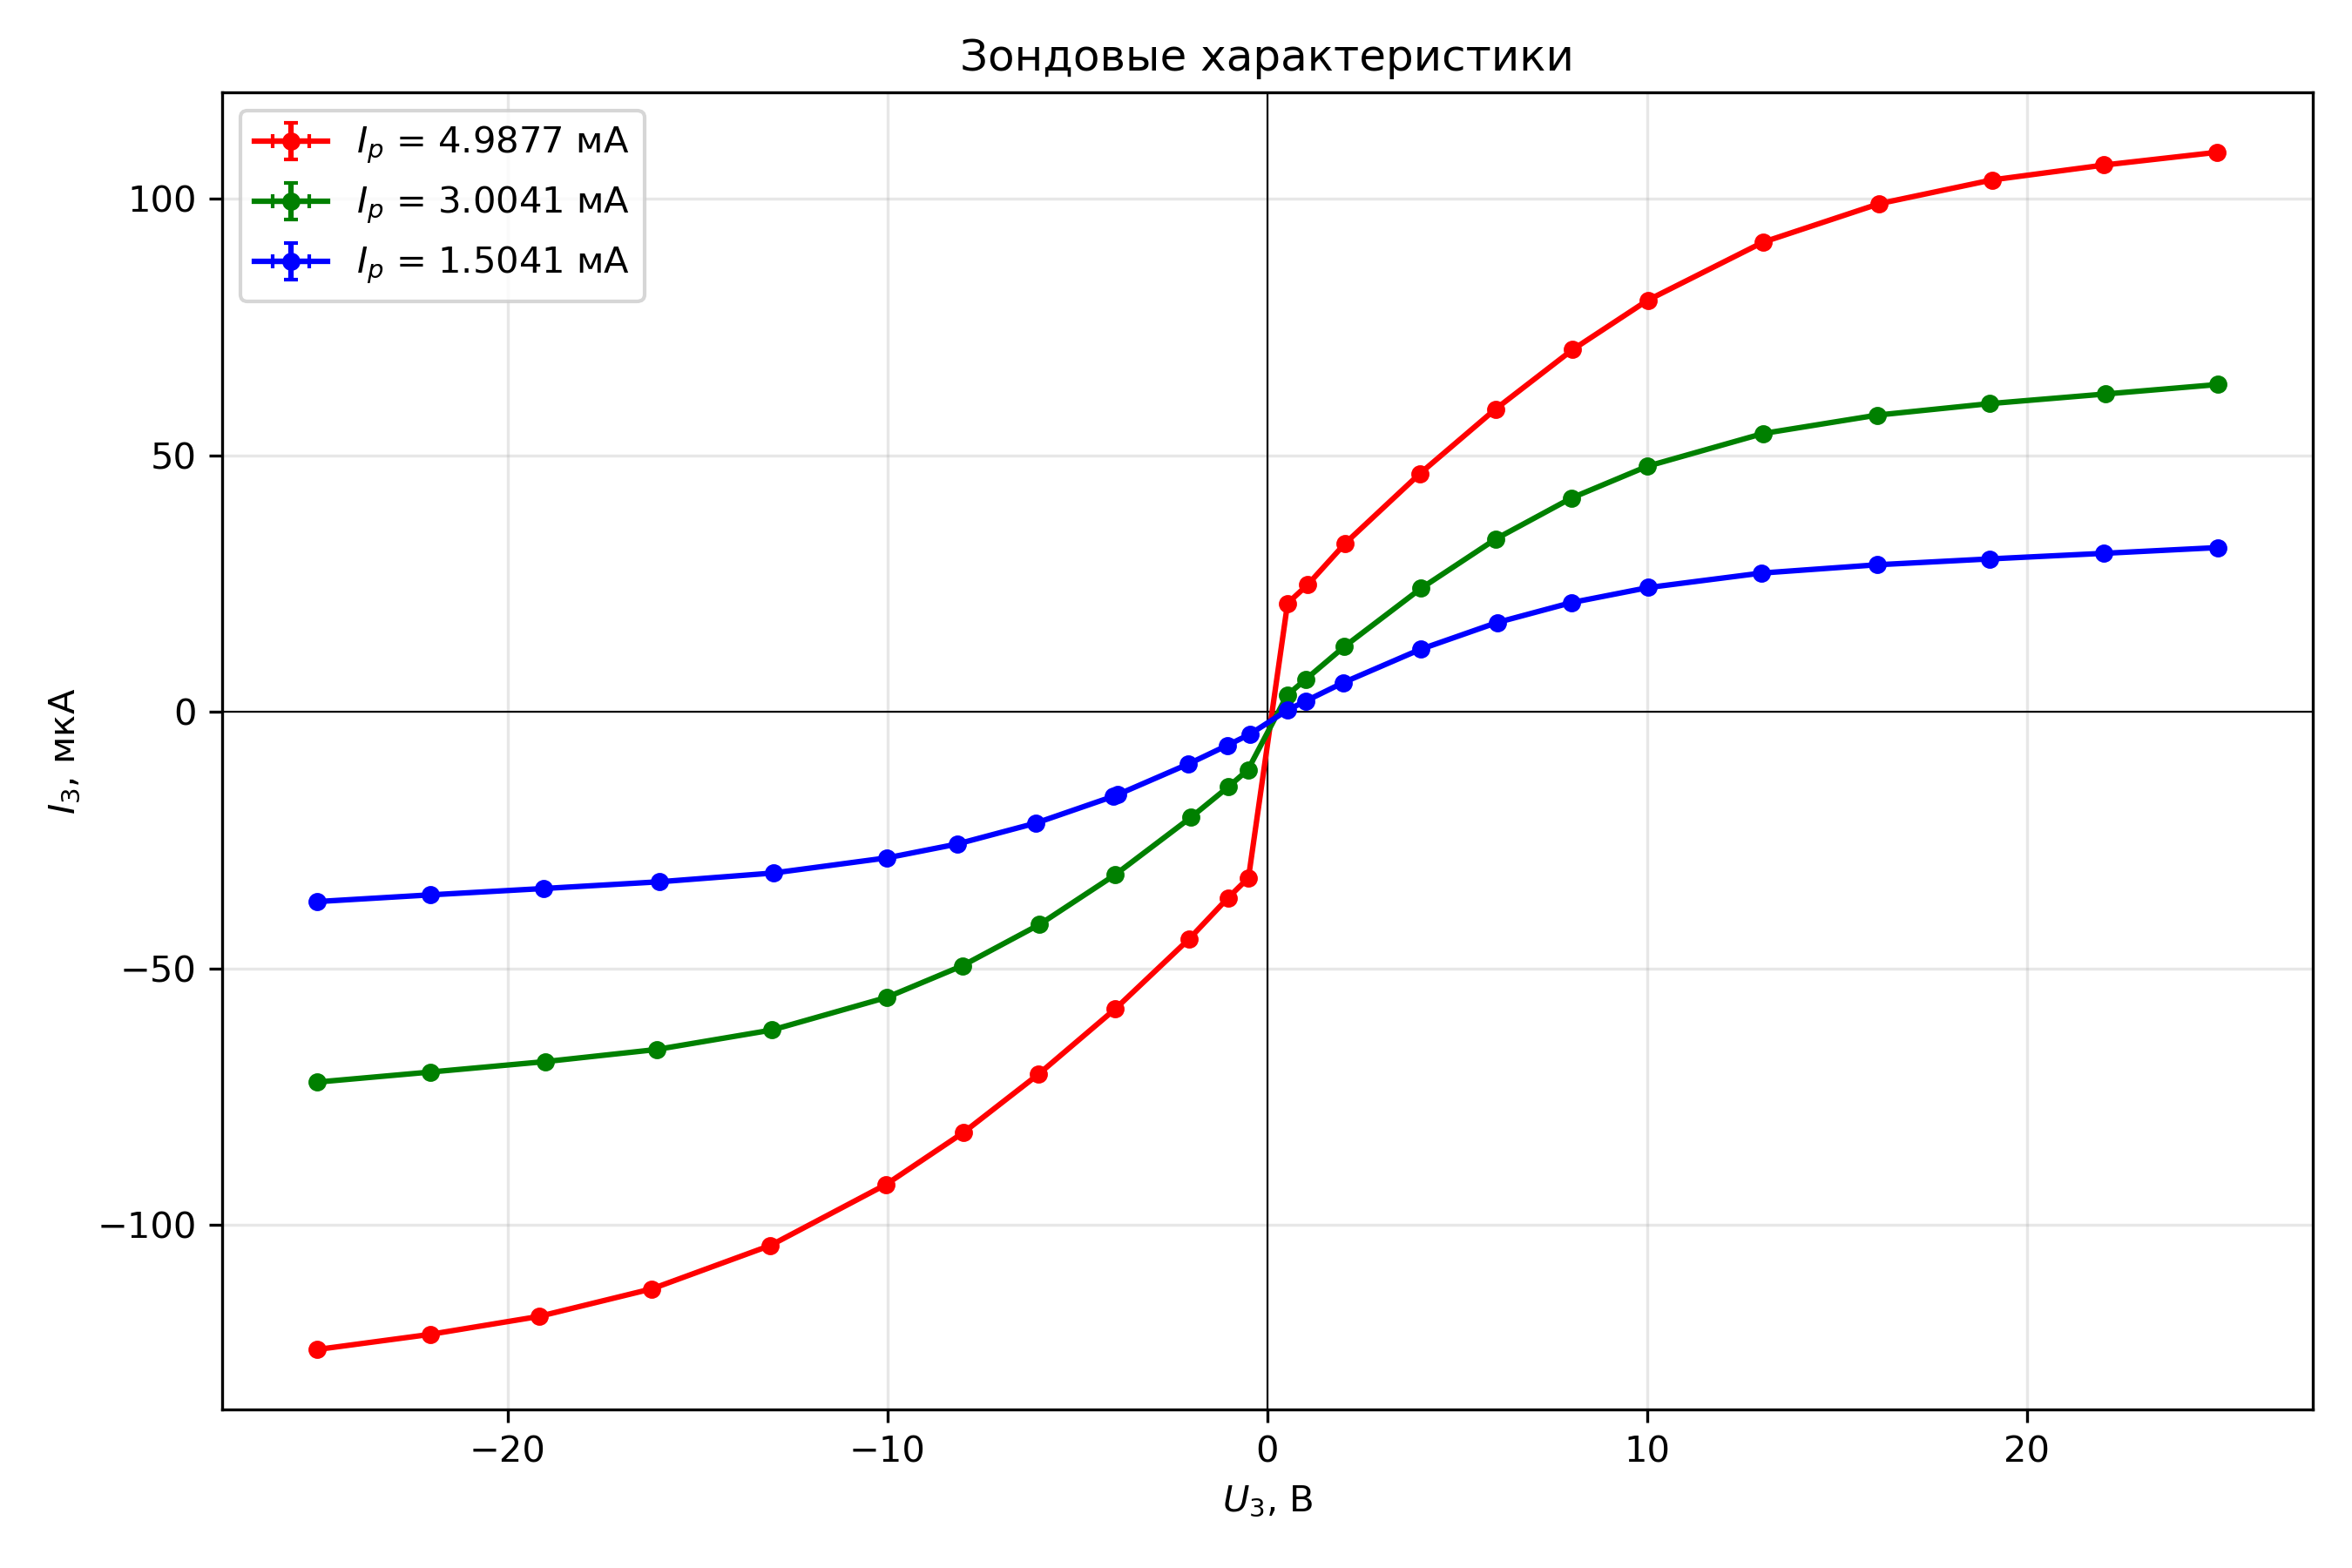
\includegraphics[width=0.85\textwidth]{probes.png}
		\caption{Семейство зондовых характеристик}
		\label{fig:probes}
	\end{figure}
	
	\subsection{Параметры плазмы}
	
	\begin{table}[h]
		\centering
		\caption{Параметры плазмы при разных токах разряда}
		\label{tab:plasma_params}
		\begin{tabular}{|c|c|c|c|c|c|c|}
			\hline
			$I_p$, мА & $k_BT_e$, эВ & $n_e$, см$^{-3}$ & $\omega_p$, рад/с & $r_{De}$, см & $r_D$, см & $N_D$ \\
			\hline
			$4{,}99$ & $0{,}9 \pm 0{,}15$ & $(8 \pm 2)\cdot 10^{12}$ & $1{,}6\cdot 10^{11}$ & $2{,}5\cdot 10^{-4}$ & $3{,}7\cdot 10^{-5}$ & 2 \\
			\hline
			$3{,}00$ & $1{,}8 \pm 0{,}27$ & $(4 \pm 1)\cdot 10^{12}$ & $1{,}1\cdot 10^{11}$ & $4{,}0\cdot 10^{-4}$ & $6{,}0\cdot 10^{-5}$ & 4 \\
			\hline
			$1{,}50$ & $2{,}6 \pm 0{,}4$ & $(1{,}7 \pm 0{,}5)\cdot 10^{12}$ & $7{,}3\cdot 10^{10}$ & $6{,}0\cdot 10^{-4}$ & $8{,}7\cdot 10^{-5}$ & 5 \\
			\hline
		\end{tabular}
	\end{table}
	
	Формулы: $\omega_p = 5{,}6\cdot 10^4\sqrt{n_e}$ (СГС);
	$r_{De} = \sqrt{k_BT_e/(4\pi n_e e^2)}$;
	$r_D \approx r_{Di} = \sqrt{k_B T_i/(4\pi n_e e^2)}$ при $T_i = 300$ К;
	$N_D = \frac{4}{3}\pi r_D^3 n_i$.
	
	\subsection{Степень ионизации}
	
	При $P = 2$ мм рт.~ст. $= 266{,}6$ Па и $T_i = 300$ К:
	\[
	n = \frac{P}{k_B T_i} \approx 6{,}4 \cdot 10^{16} \ \text{см}^{-3}.
	\]
	\[
	\alpha = \frac{n_e}{n} \approx (1{,}3 \pm 0{,}4)\cdot 10^{-4} \approx 0{,}013\,\%.
	\]
	
	\subsection{Зависимости $T_e(I_p)$ и $n_e(I_p)$}
	
	\begin{figure}[h]
		\centering
		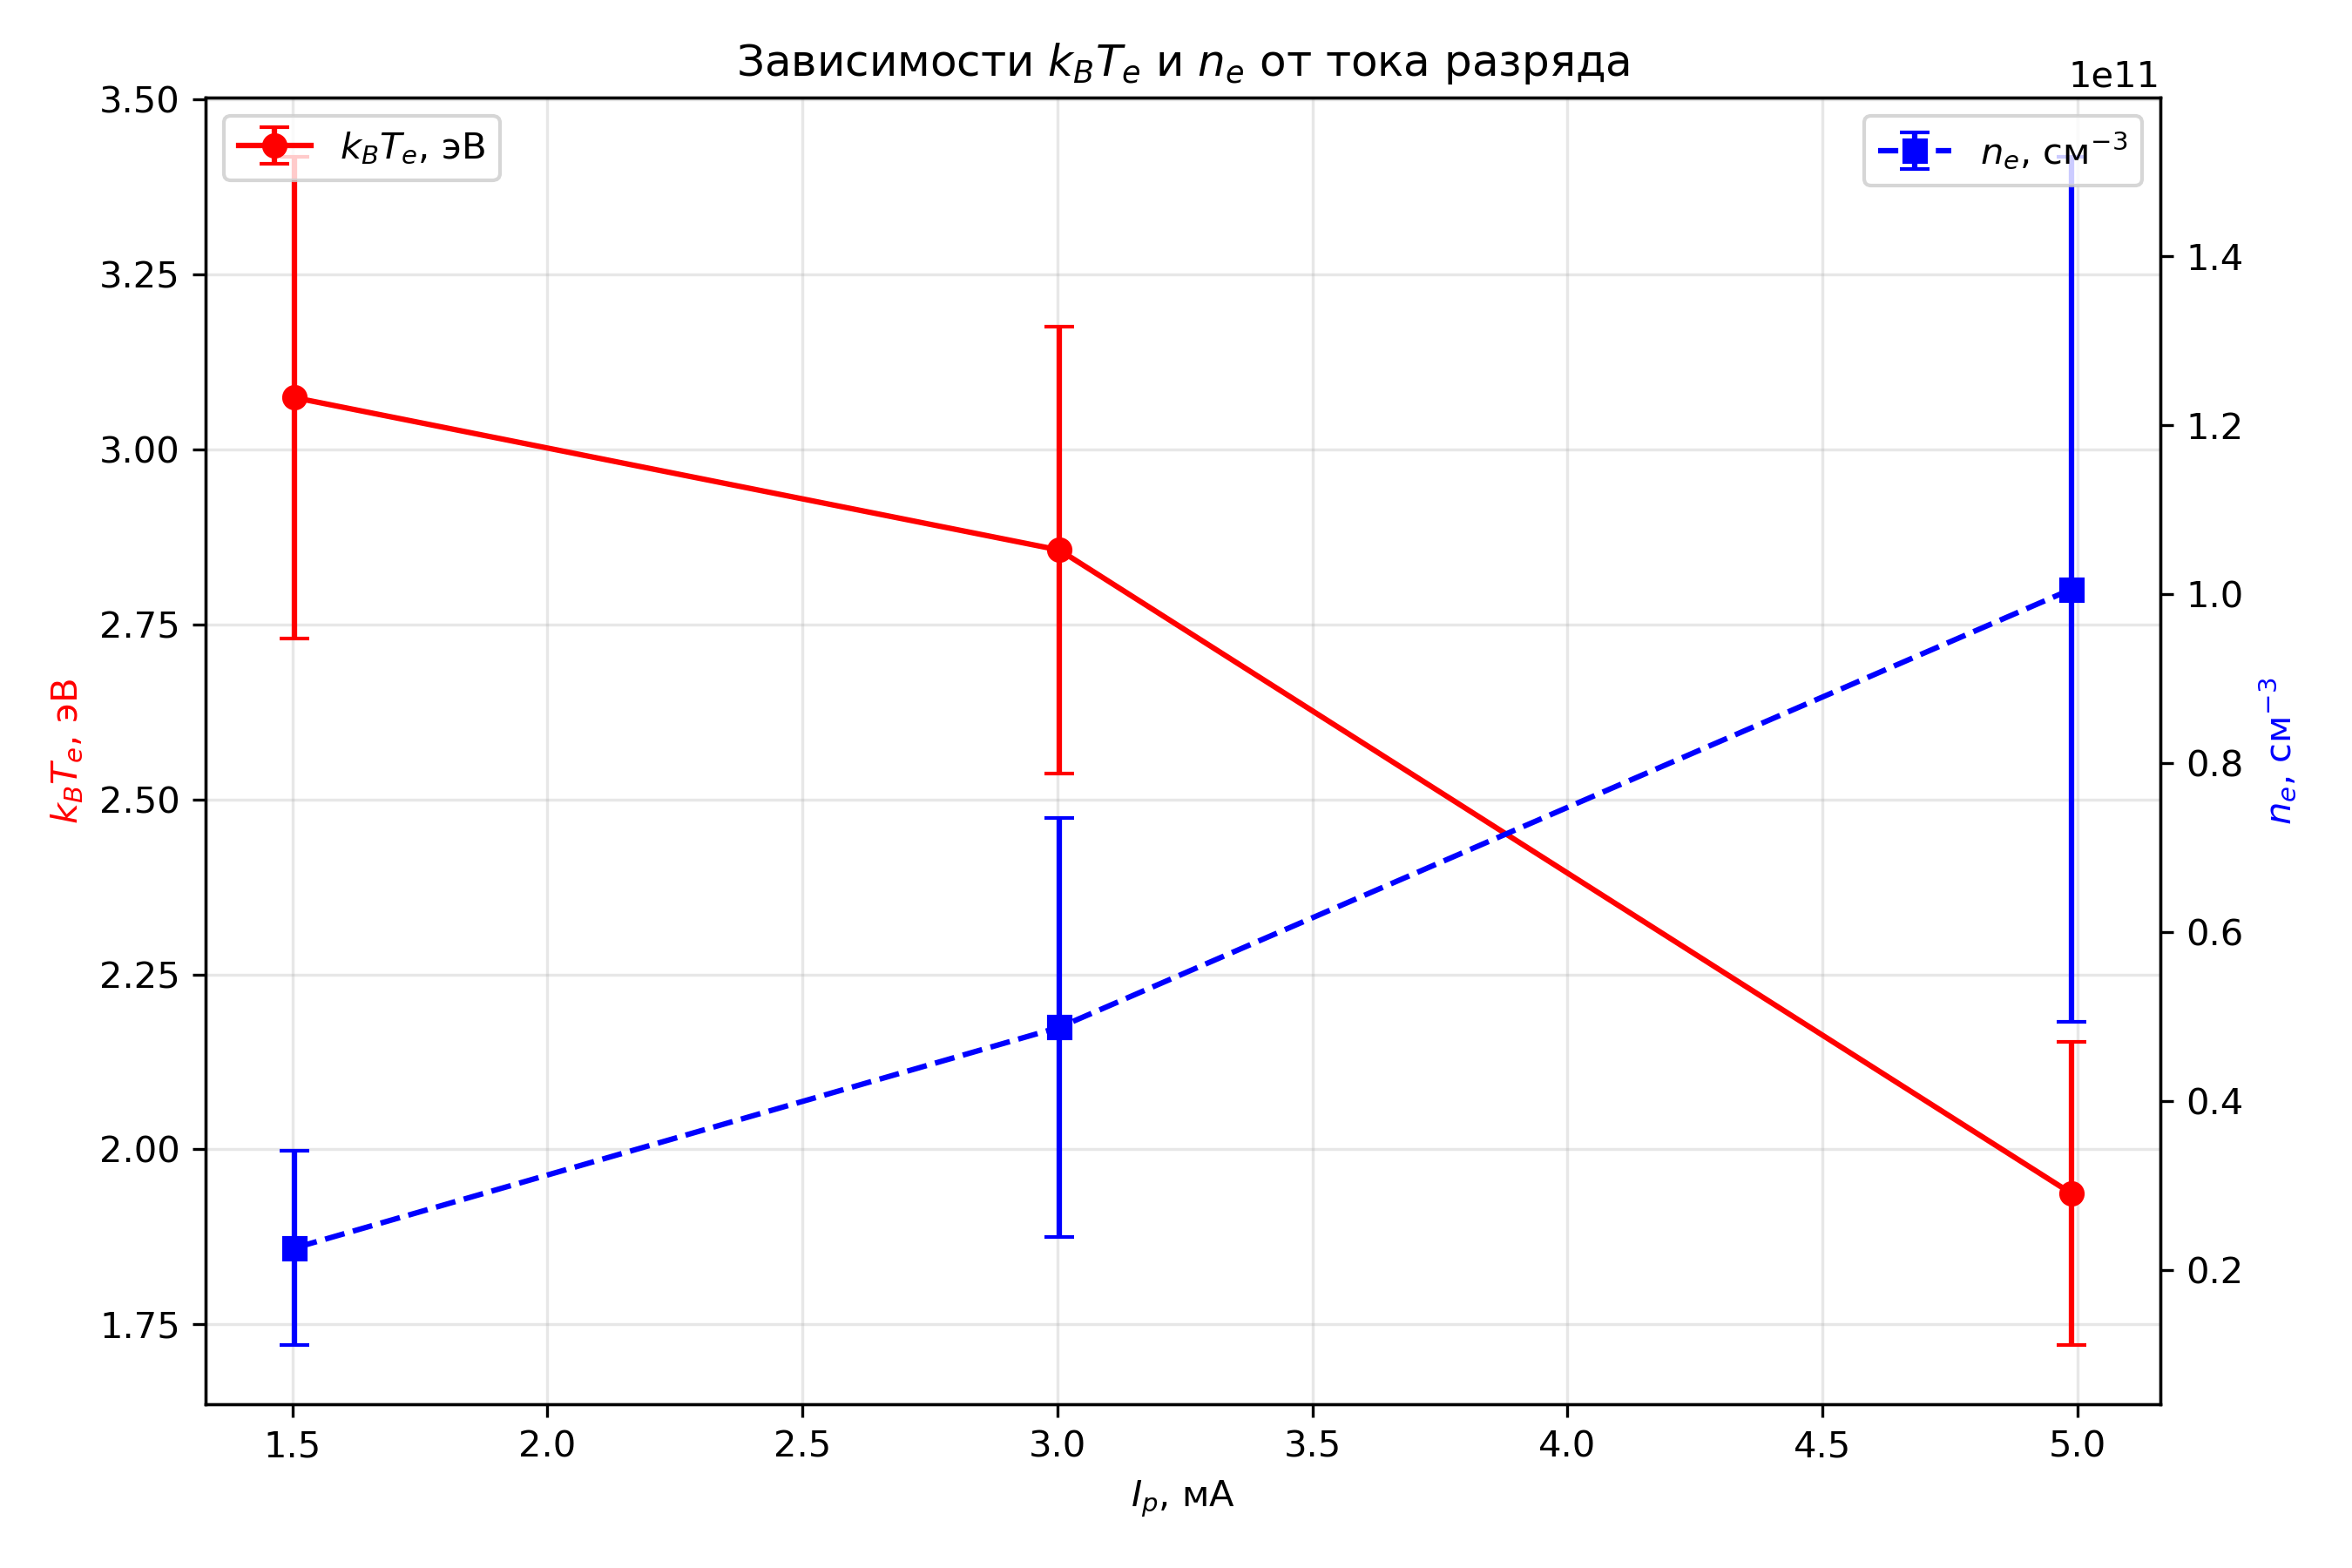
\includegraphics[width=0.85\textwidth]{plasma_params.png}
		\caption{Зависимости $k_BT_e$ и $n_e$ от тока разряда}
		\label{fig:plasma_params}
	\end{figure}
	
	\section{Оценка погрешностей}
	
	\textbf{Прямые измерения (по последнему значащему знаку):}
	\begin{itemize}
		\item Ток зонда: $\delta I_3 = 0{,}01$ мкА;
		\item Напряжение на зонде: $\delta U_3 = 0{,}001$ В;
		\item Ток разряда: $\delta I_p = 0{,}0001$ мА;
		\item Напряжение разряда (после $\times 10$): $\delta U_p = 0{,}1$ В;
		\item Напряжение зажигания: $\delta U_{\text{заж}} = 0{,}001$ В;
		\item Диаметр и длина зонда: $\delta d = \delta l = 0{,}1$ мм.
	\end{itemize}
	
	\textbf{Косвенные погрешности:}
	\begin{itemize}
		\item $\delta I_{in} \approx 5\%$ (аппроксимация асимптот);
		\item $\delta (dI/dU)|_0 \approx 10\%$;
		\item $\delta k_BT_e \approx 15\%$;
		\item $\delta n_e \approx 20\%$ (формула Бома $+$ неопределённость $S$ зонда);
		\item $\delta R_{\text{диф}} \approx 0{,}5\%$ (определяется погрешностями прямых измерений $U_p$, $I_p$).
	\end{itemize}
	
	\section{Выводы}
	
	\begin{enumerate}
		\item Измерена ВАХ тлеющего разряда в неоне. Напряжение зажигания $U_{\text{заж}} = (2140{,}000 \pm 0{,}001)$ В. После зажигания напряжение резко падает и далее лежит в диапазоне $185$--$350$ В. Потенциал гашения ($\sim 186$ В) меньше $U_{\text{заж}}$ — наблюдается гистерезис. Максимальное дифференциальное сопротивление $R_{\text{диф}} \approx 130$ кОм (в области поднормального тлеющего разряда, $I_p \approx 1{,}1$ мА).
		
		\item Построены зондовые характеристики двойного зонда при $I_p = 4{,}99$, $3{,}00$ и $1{,}50$ мА. Ионные токи насыщения: $I_{in} = (90 \pm 5)$, $(53 \pm 3)$ и $(26 \pm 2)$ мкА.
		
		\item Температуры электронов:
		\[
		k_BT_e = (0{,}9 \pm 0{,}15);\ (1{,}8 \pm 0{,}27);\ (2{,}6 \pm 0{,}4) \ \text{эВ}.
		\]
		Температура падает с ростом тока — типично для тлеющего разряда (при больших токах растут потери энергии на ионизацию).
		
		\item Концентрации электронов: $n_e \sim (8 \pm 2)\cdot 10^{12}$, $(4 \pm 1)\cdot 10^{12}$ и $(1{,}7 \pm 0{,}5)\cdot 10^{12}$ см$^{-3}$. Соответствующие плазменные частоты $\omega_p \sim 10^{11}$ рад/с, поляризационные длины $r_{De} \sim 10^{-4}$ см, дебаевские радиусы $r_D \sim 10^{-5}$ см.
		
		\item Число частиц в дебаевской сфере $N_D \approx 2$--$5$ — плазма близка к идеальной.
		
		\item Степень ионизации $\alpha \sim 10^{-4}$ — слабоионизованная газоразрядная плазма.
		
		\item Обнаружена зависимость параметров плазмы от тока разряда: температура электронов падает, концентрация растёт.
	\end{enumerate}
	
	\newpage
	\section{Приложения}
	
	\begin{figure}[h]
		\centering
		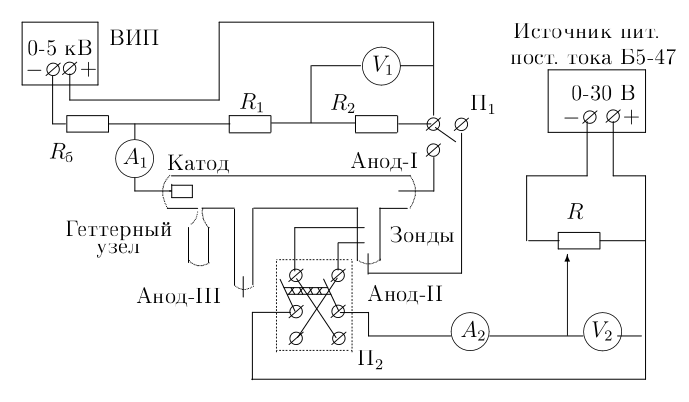
\includegraphics[width=0.9\textwidth]{setup.png}
		\caption*{Приложение 1. Схема установки}
	\end{figure}
	
	\begin{figure}[h]
		\centering
		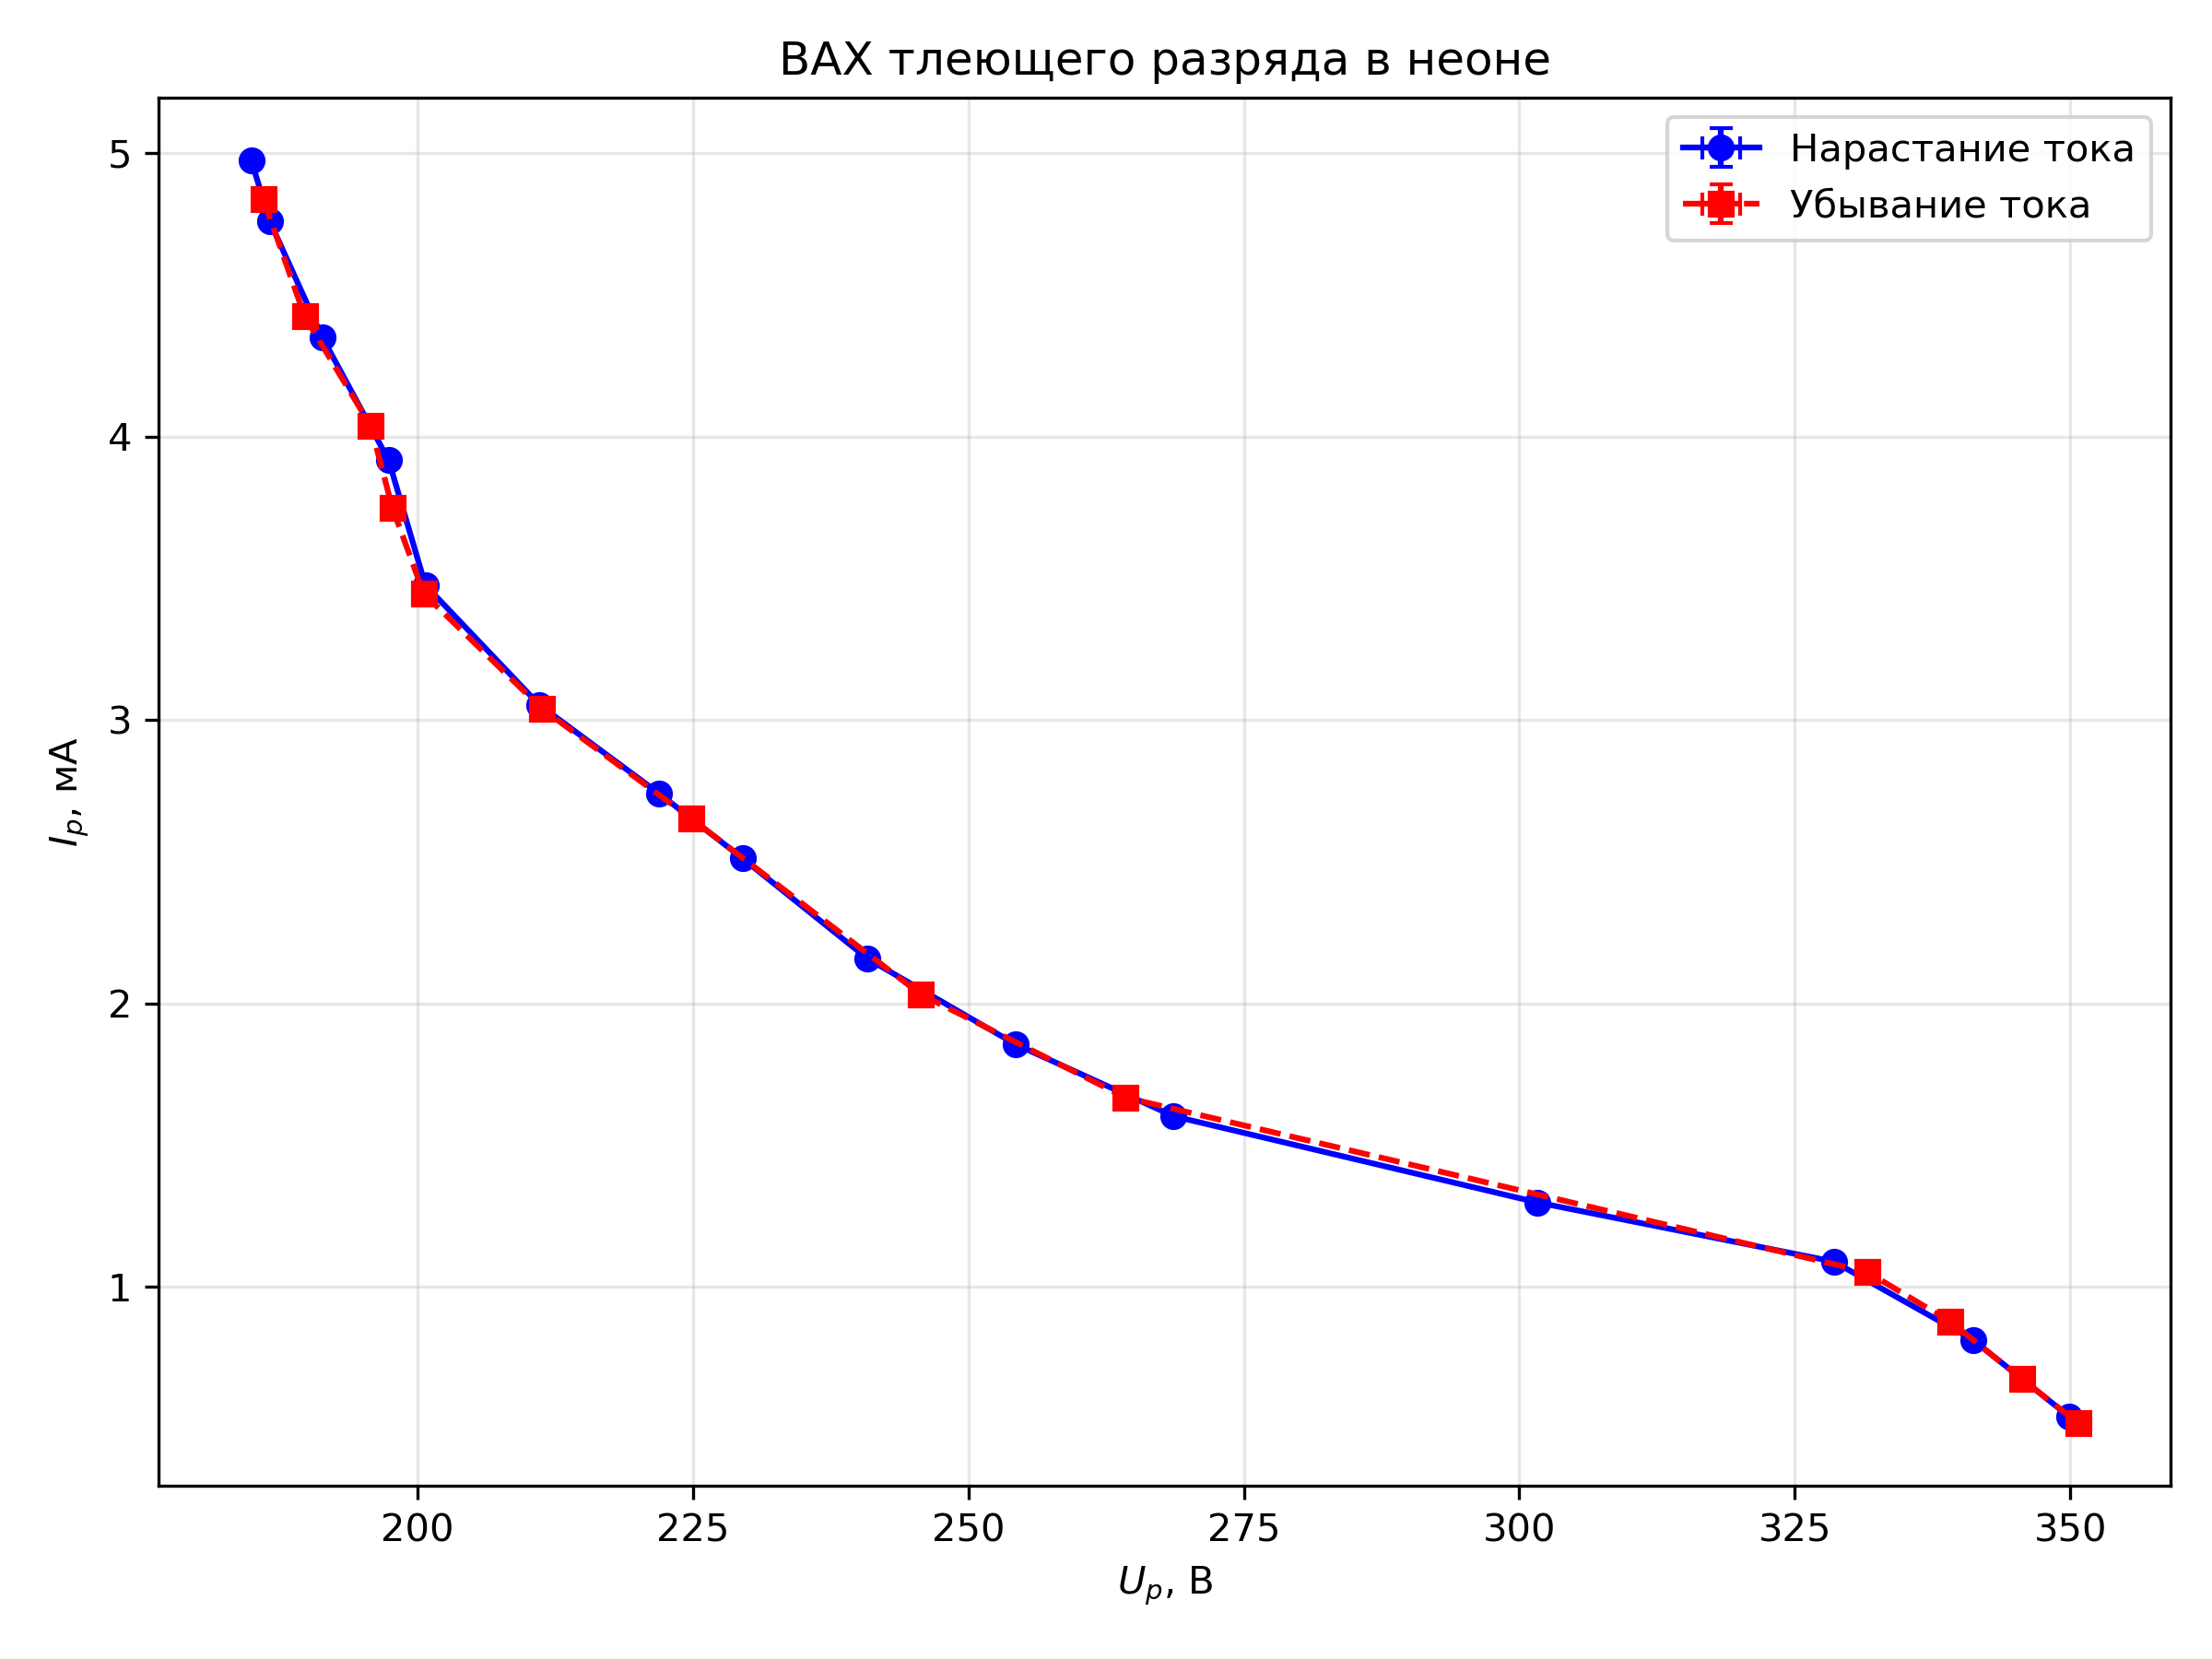
\includegraphics[width=0.85\textwidth]{vac.png}
		\caption*{Приложение 2. ВАХ тлеющего разряда}
	\end{figure}
	
	\begin{figure}[h]
		\centering
		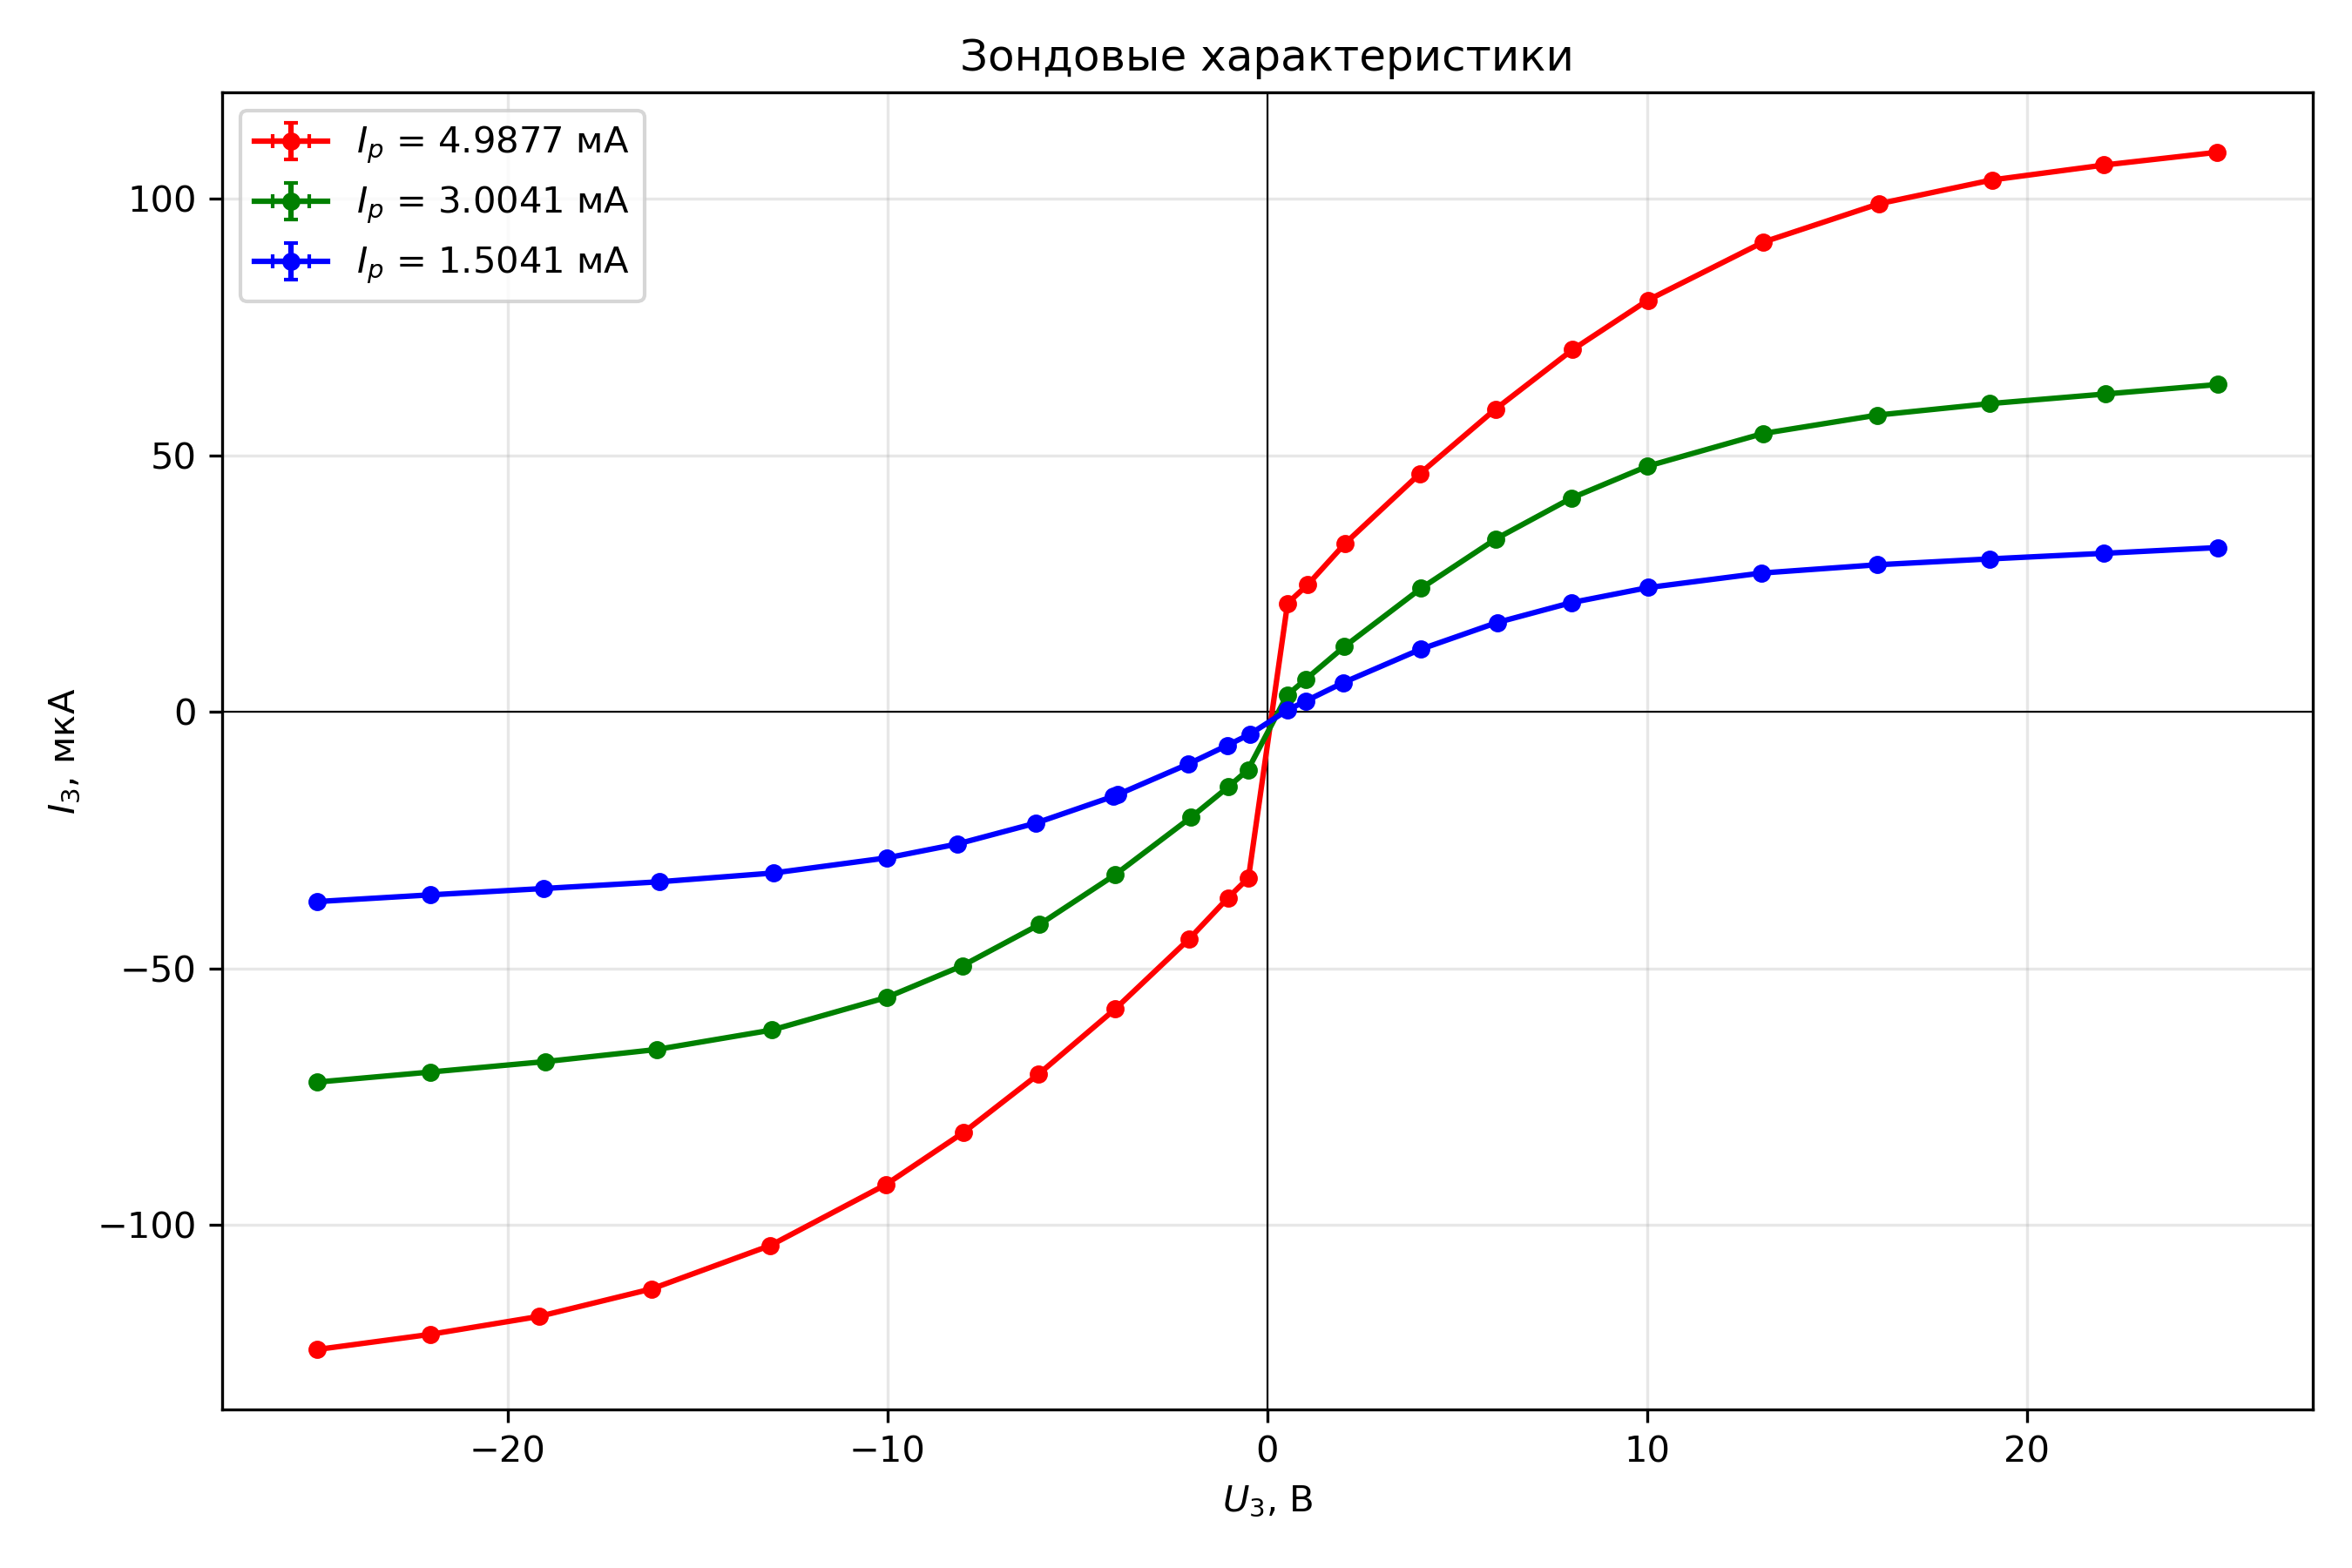
\includegraphics[width=0.85\textwidth]{probes.png}
		\caption*{Приложение 3. Семейство зондовых характеристик}
	\end{figure}
	
	\begin{figure}[h]
		\centering
		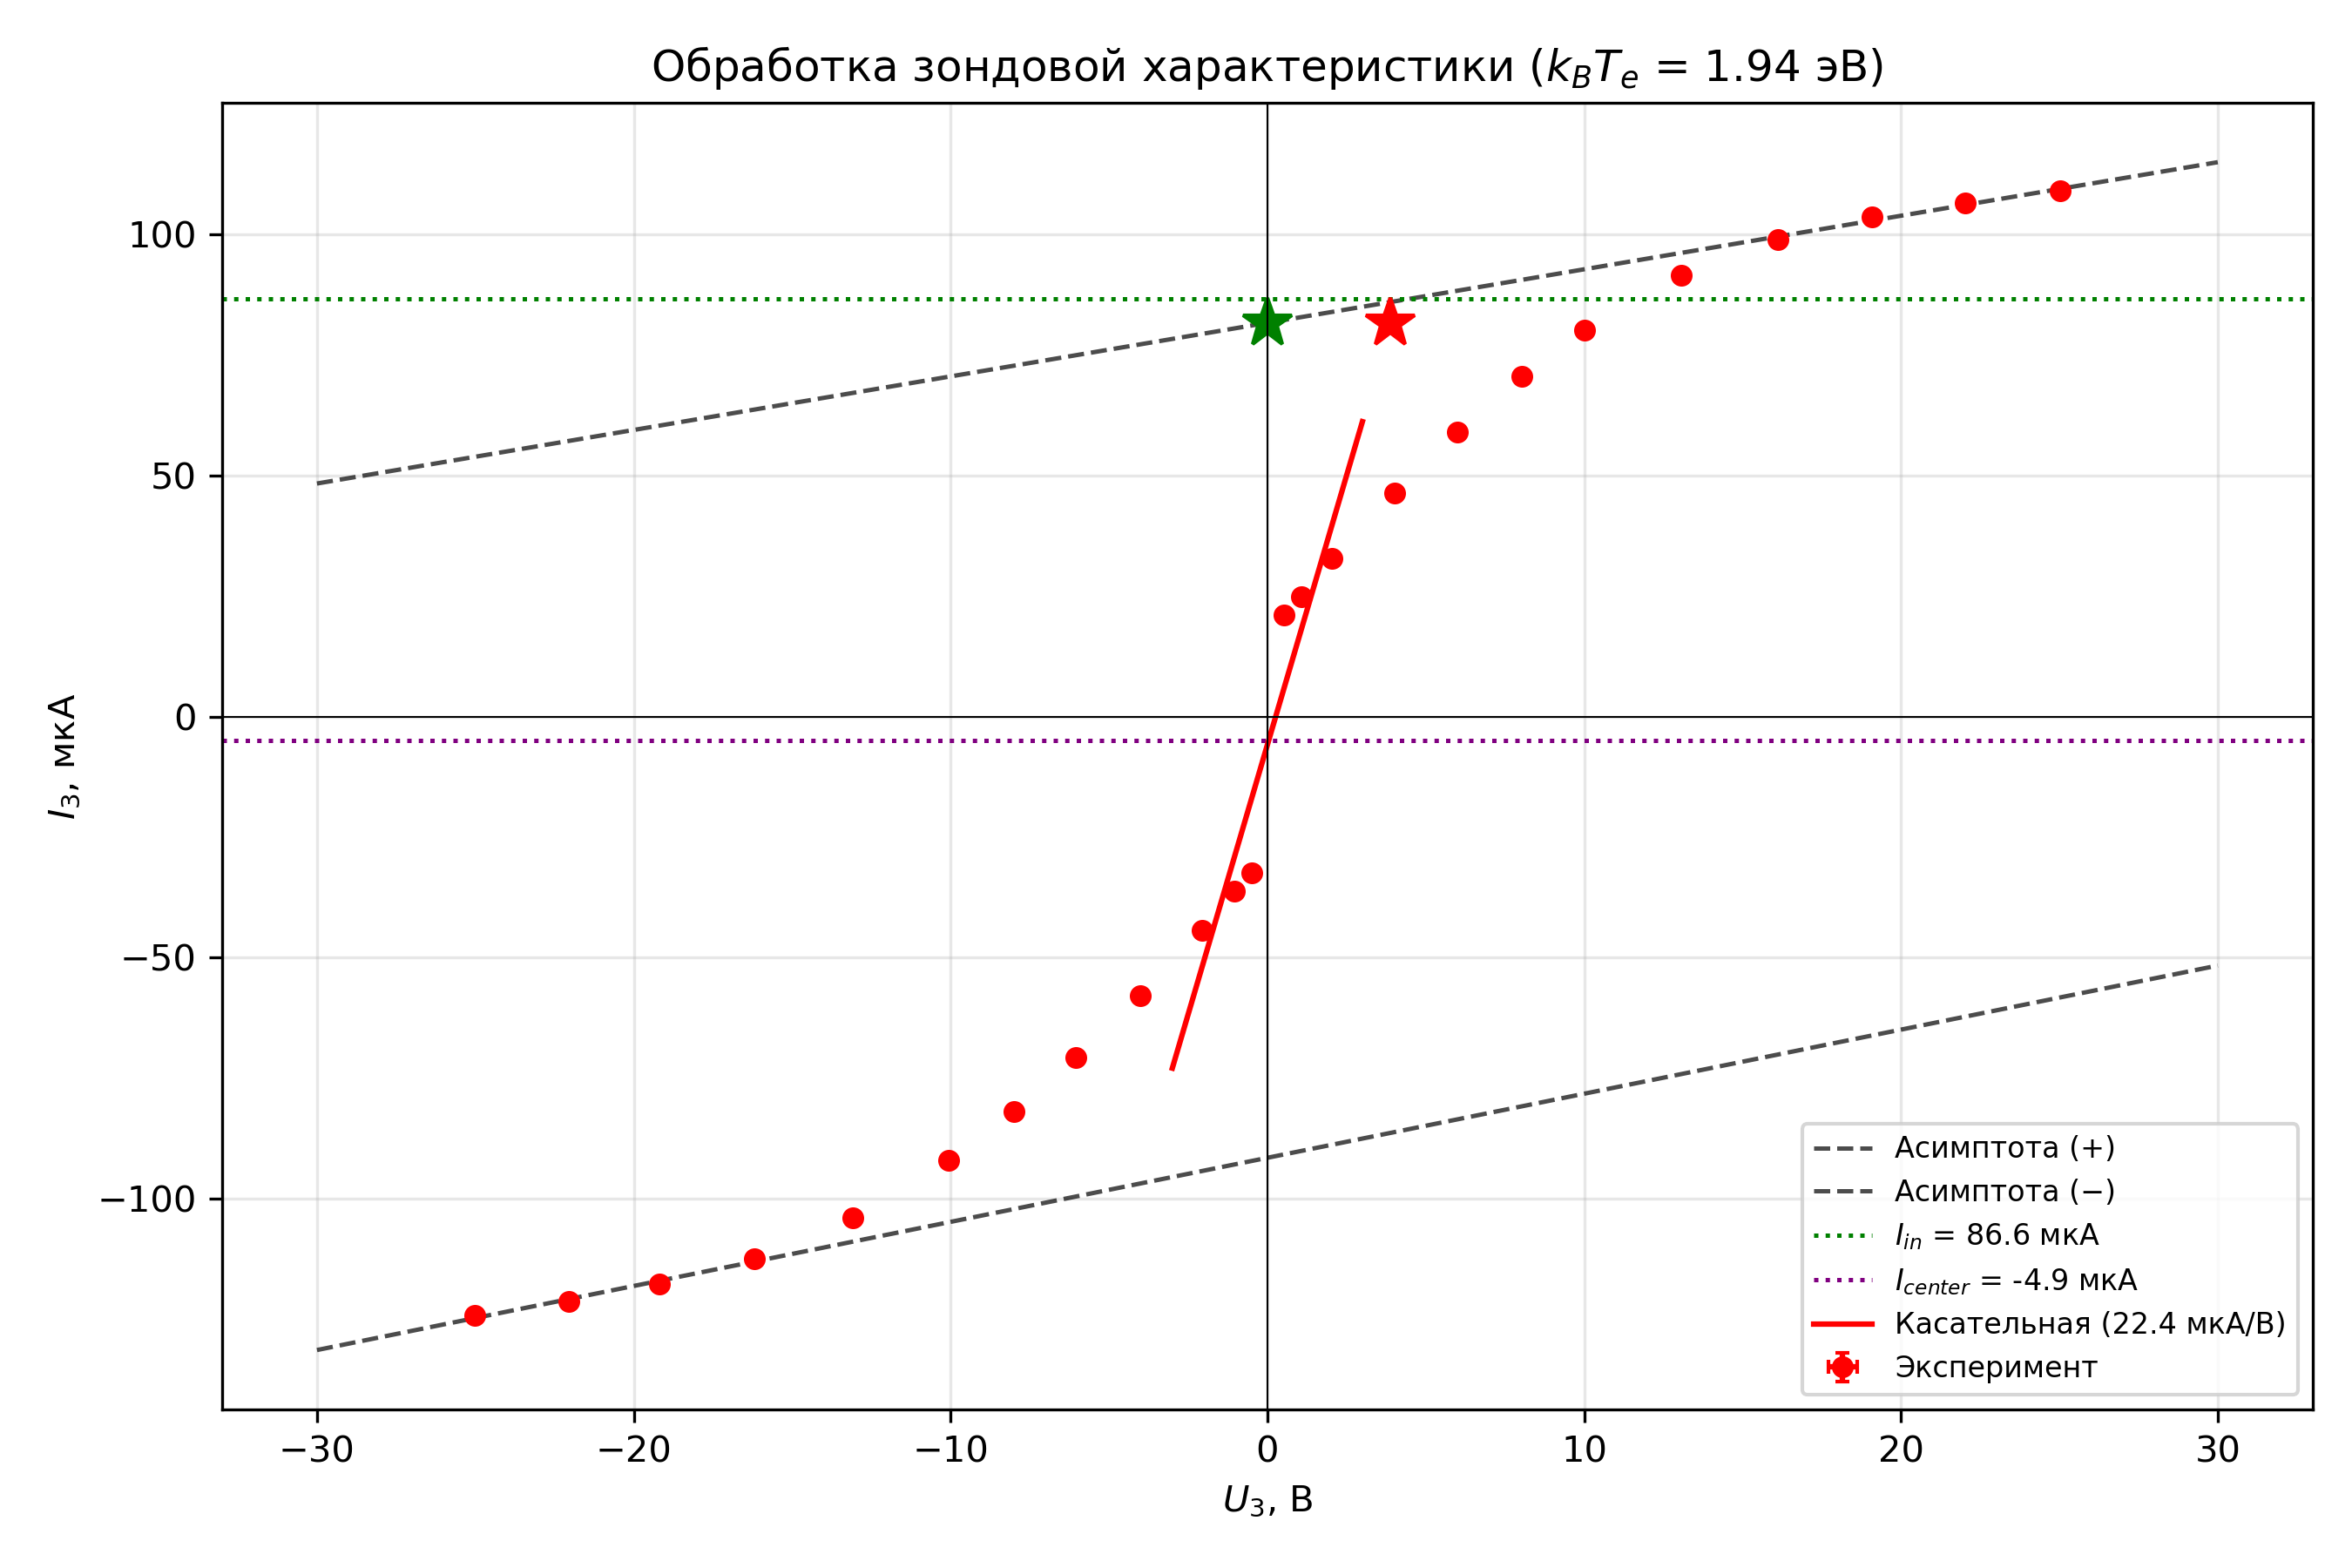
\includegraphics[width=0.9\textwidth]{probe_analysis.png}
		\caption*{Приложение 4. Обработка зондовой характеристики}
	\end{figure}
	
	\begin{figure}[h]
		\centering
		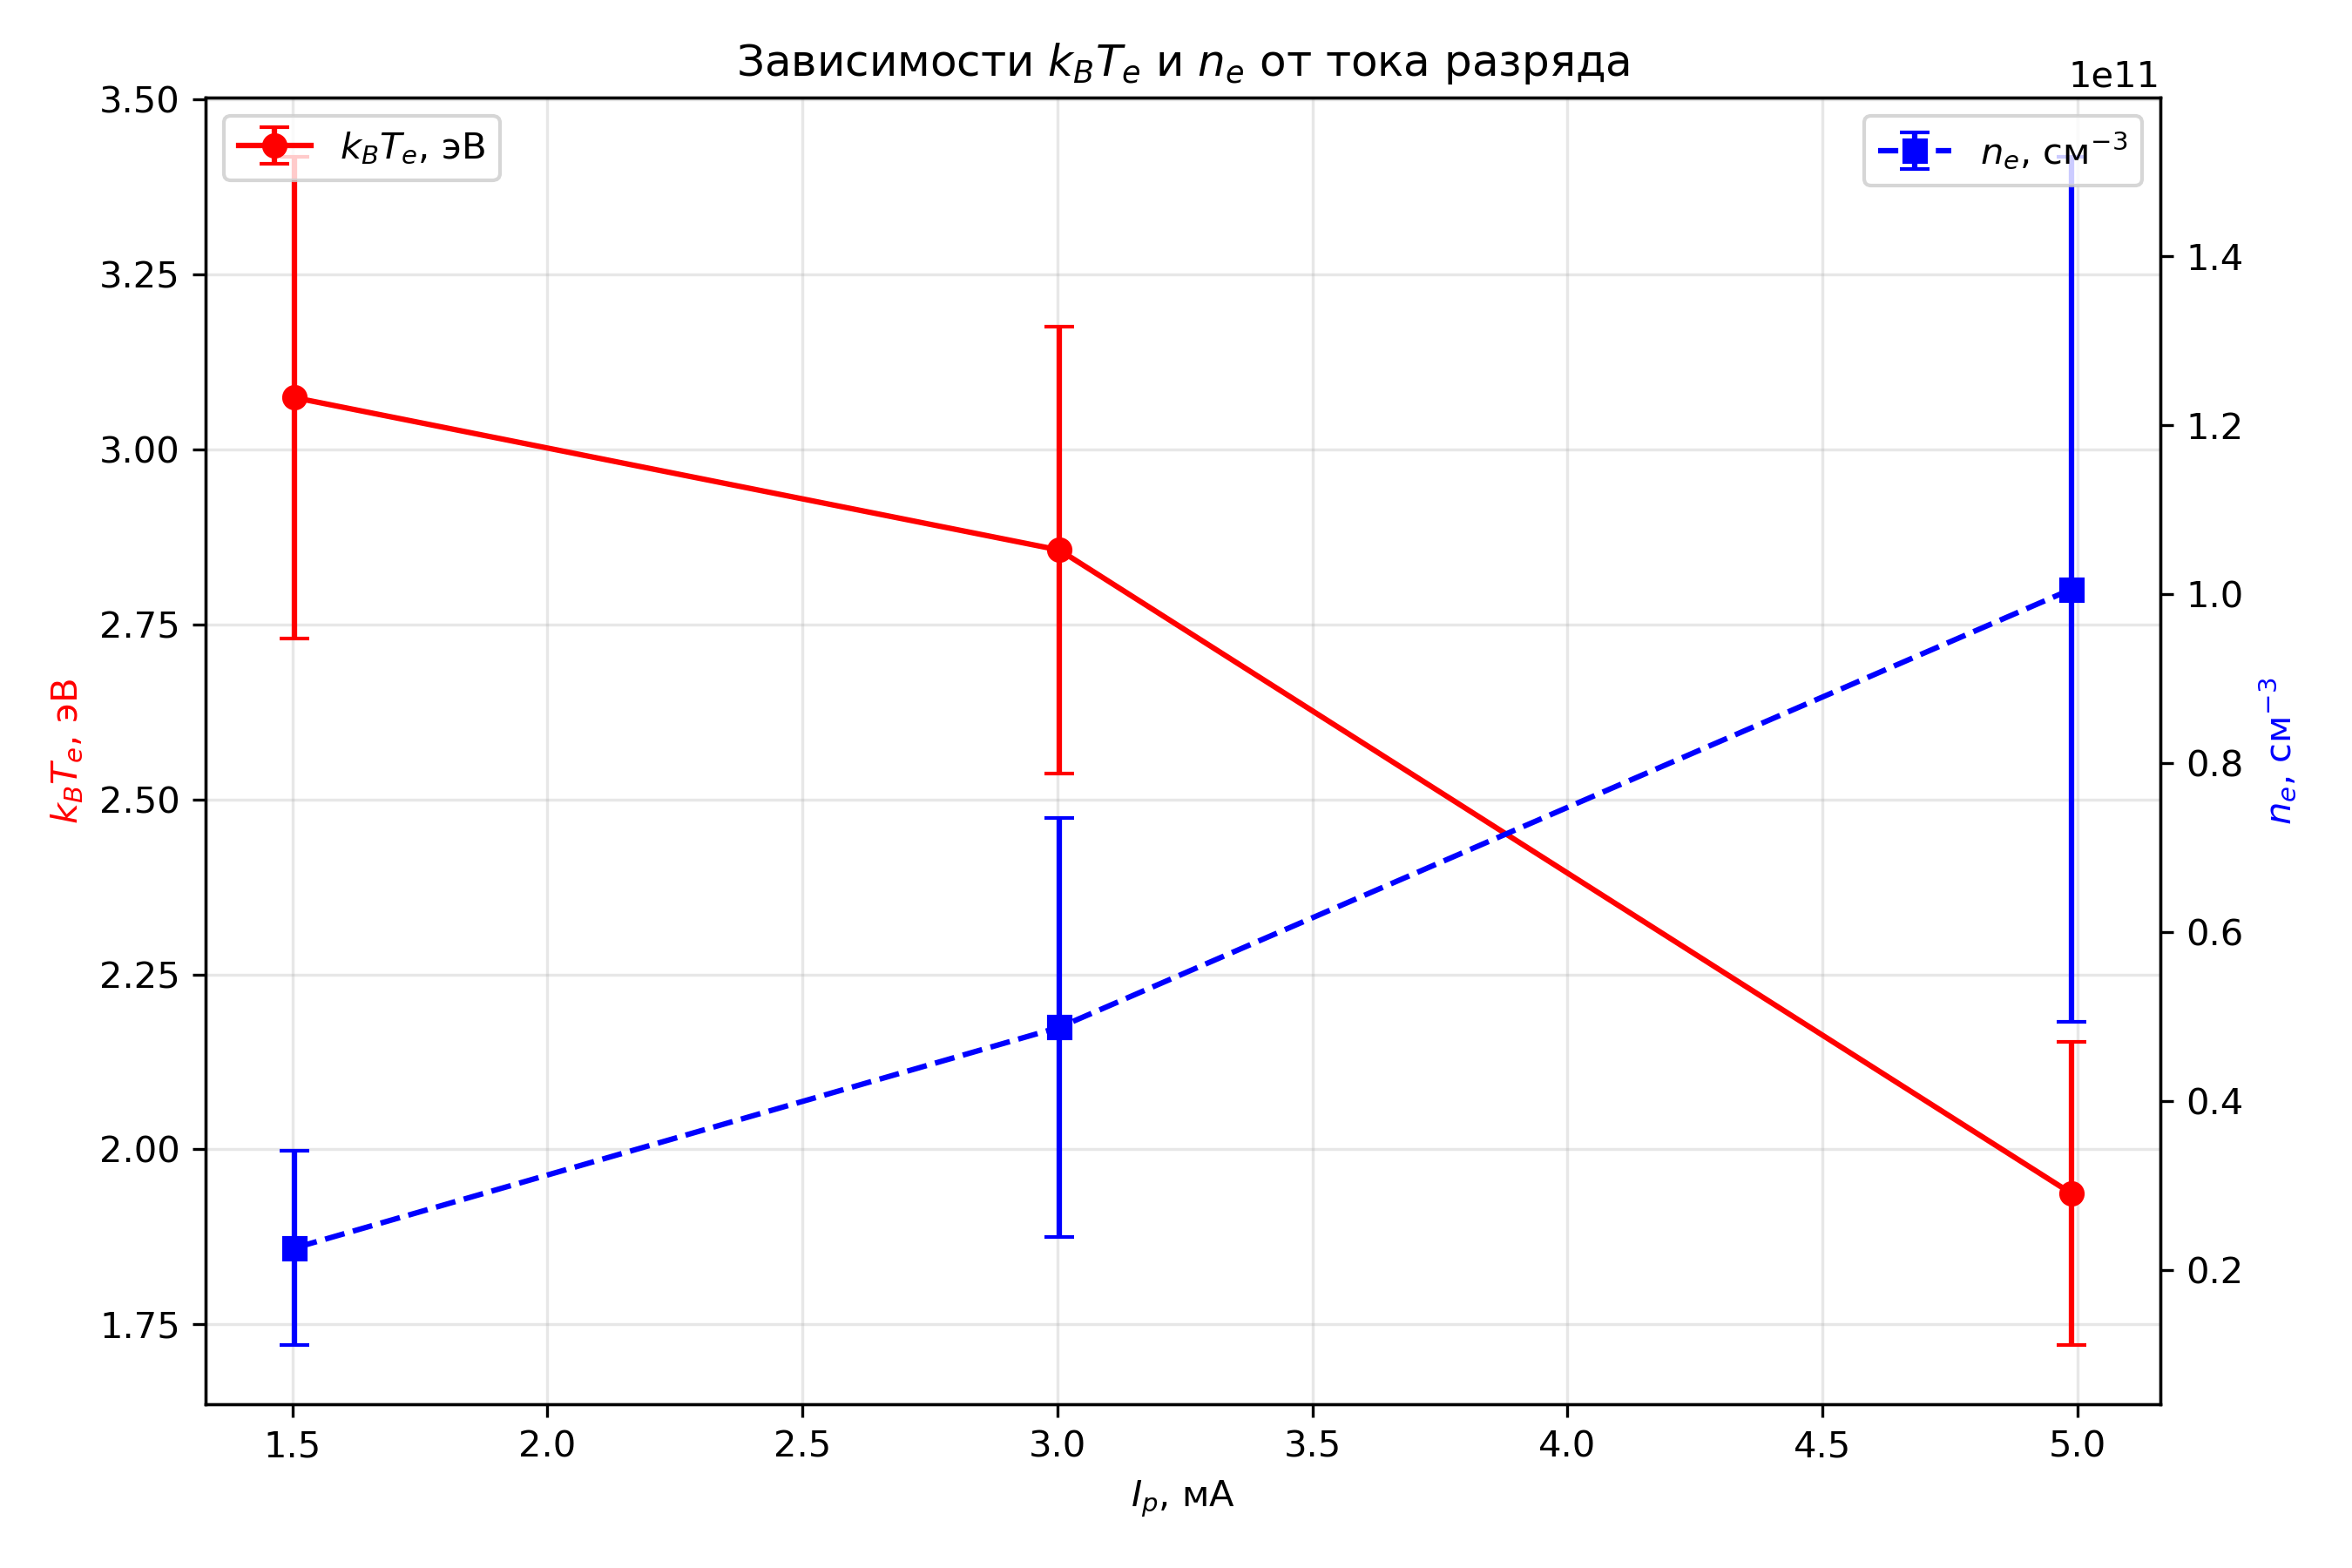
\includegraphics[width=0.85\textwidth]{plasma_params.png}
		\caption*{Приложение 5. Зависимости $k_BT_e$ и $n_e$ от тока разряда}
	\end{figure}
	
\end{document}